\documentclass{article}

\usepackage{graphicx}
\usepackage{rotating}
\usepackage{amsmath}
\usepackage{amssymb}
\usepackage{fancyhdr}
\usepackage{listings}
\usepackage{lscape}
\usepackage{multirow}
\usepackage{color}
\usepackage{amsfonts}
\usepackage{textcomp}
\usepackage{float}
\usepackage{longtable}
\usepackage{booktabs}
\usepackage[sorting=none]{biblatex}
\usepackage[margin=1in]{geometry}
\usepackage[font={small,it}]{caption}
\usepackage[table,xcdraw]{xcolor}
\usepackage{placeins}
\usepackage{xepersian}





%\DeclareMathOperator*{\btie}{\bowtie}
\addbibresource{bibliography.bib}
\settextfont[Scale=1.2]{B-NAZANIN.TTF}
\setlatintextfont[Scale=1]{Times New Roman}
\renewcommand{\baselinestretch}{1.5}
\pagestyle{fancy}
\fancyhf{}
\rhead{تکلیف تئوری سوم درس کامپایلر}
\lhead{\thepage}
\rfoot{علیرضا ابره فروش}
\lfoot{9816603}
\renewcommand{\headrulewidth}{1pt}
\renewcommand{\footrulewidth}{1pt}
%%%%%%%%%%
\lstset
{
    language=[latex]tex,
    basicstyle=\ttfamily,
    commentstyle=\color{black},
    columns=fullflexible,
    keepspaces=true,
    upquote=true,
    showstringspaces=false,
    morestring=[s]\\\%,
    stringstyle=\color{black},
}
%%%%%%%%%%
%beginMatlab
\definecolor{mygreen}{RGB}{28,172,0} % color values Red, Green, Blue
\definecolor{mylilas}{RGB}{170,55,241}
%endMatlab
\begin{document}
%beginMatlab
\lstset{language=Matlab,%
    %basicstyle=\color{red},
    breaklines=true,%
    morekeywords={matlab2tikz},
    keywordstyle=\color{blue},%
    morekeywords=[2]{1}, keywordstyle=[2]{\color{black}},
    identifierstyle=\color{black},%
    stringstyle=\color{mylilas},
    commentstyle=\color{mygreen},%
    showstringspaces=false,%without this there will be a symbol in the places where there is a space
    numbers=left,%
    numberstyle={\tiny \color{black}},% size of the numbers
    numbersep=9pt, % this defines how far the numbers are from the text
    emph=[1]{for,end,break},emphstyle=[1]\color{red}, %some words to emphasise
    %emph=[2]{word1,word2}, emphstyle=[2]{style},    
}
%endMatlab
\begin{titlepage}
\begin{center}

\includegraphics[width=0.4\textwidth]{figures/IUT Logo.png}\\
        
\LARGE
\textbf{دانشگاه صنعتی اصفهان}\\
\textbf{دانشکده مهندسی برق و کامپیوتر}\\
        
\vfill
        
\huge
\textbf{عنوان: تکلیف چهارم درس ریزپردازنده}\\
        
\vfill
        
\LARGE
\textbf{نام و نام خانوادگی: علیرضا ابره فروش}\\
\textbf{شماره دانشجویی: 9816603}\\
\textbf{نیم\,سال تحصیلی: پاییز 1400}\\
\textbf{مدرّس: دکتر عارف کریمی افشار}\\
\end{center}
\end{titlepage}


%\tableofcontents
\newpage

\section{}%1
\subsection{آ}
نادرست-چون
$
LR(1) \subset LR(2)
$
است و نه برعکس. به مثال مقابل توجه کنید.\\
\begin{latin}
$\\
E \longrightarrow  X_1 Y a | X_2 Y b \\
X_1 \longrightarrow  x \\
X_2 \longrightarrow  x \\
Y \longrightarrow  y
$
\end{latin}
این گرامر $LR(2)$ است ولی $LR(1)$ نیست.

\subsection{ب}
درست-به ازای هر گرامر $LR(k)$ به طوری که $k \ge 2$، یک گرامر $LR(1)$ وجود دارد که زبان یکسانی را توصیف می‌کند. توجه شود که پارسرهای این دو زبان لزوما یکسان نمی‌باشند.

\subsection{ج}
درست-الگوریتم \lr{CYK} هر رشته‌ی به طول $n$ای را در هر گرامر \lr{Context-free}ای در زمان $O(n^3)$ تجزیه می‌کند.

\subsection{د}
نادرست-به مثال مقابل توجه کنید.\\
\begin{latin}
$\\
S \longrightarrow  L = R \\
S \longrightarrow R \\
L \longrightarrow * R \\
L \longrightarrow id \\
R \longrightarrow L
$
\end{latin}
این گرامر غیرمبهم است ولی $SLR(1)$ نیست.


\section{}%2
\subsection{}
\subsubsection{قدرت}
\begin{latin}
$
SLR(1) \le LALR(1) \le LR(1) \le LR(k)
$
\end{latin}
\subsubsection{پیاده‌سازی}
\begin{latin}
$
SLR(1) = LALR(1) < LR(1) < LR(k)
$
\end{latin}
میزان پیچیدگی حافظه و پیاده‌سازی به طور نمایی با زیاد شدن $k$ زیاد می‌شود.


\section{}%3
تعداد استیت‌ها در $SLR(1)$ و $LALR(1)$ برابر است و بسیار کمتر از $LR(1)$ است.
\begin{latin}
$
n_1 > n_2 = n_3
$
\end{latin}


\section{}%4
حداكثر تعداد \lr{reduce}هايي كه مي‌تواند توسط يك تجزيه كننده‌ی پايين به بالا براي يك گرامر بدون قانون‌هاي اپسيلون يا واحد براي تجزيه‌ی رشته‌اي به طول $n$ وجود داشته باشد برابر است با $2n-1$. در حالت حداکثر هر \lr{reduction} یا به صورتِ $X \longrightarrow x$ است و یا به صورتِ $X \longrightarrow YZ$ (که $x$ ترمینال، و $X$ و $Y$ و $Z$ غیرترمینال است) توجه شود که تعداد غیرترمینال‌های \lr{RHS}های \lr{reduction}ها در حالت حداکثری باید کمینه باشد و با توجه به شرط مسئله 1 هم نباشد. پس در نهایت در حالت حداکثری به ازای هر سمبل رشته 1 \lr{reduction} خواهیم داشت (که به صورتِ $X \longrightarrow x$ است) و $n-1$ \lr{reduction} هم به صورتِ  $X \longrightarrow YZ$ خواهیم داشت. پس در کل تعداد \lr{reduction}ها حداکثر برابر با $2n-1$ است. به مثال زیر توجه کنید.
\begin{latin}
$\\
S \longrightarrow  AB \\
A \longrightarrow XY \\
B \longrightarrow ZW \\
X \longrightarrow x \\
Y \longrightarrow y \\
Z \longrightarrow z \\
W \longrightarrow w
$
\end{latin}
برای رشته‌ی $xyzw$ داریم:
\begin{latin}
$\\
S \longrightarrow  AB \longrightarrow XYB \longrightarrow XYZW \longrightarrow xYZW \longrightarrow xyZW \longrightarrow xyzW \longrightarrow xyzw
$
\end{latin}
که معادل 7 تا \lr{reduction} است.


\section{}%5
\subsection{}
\subsubsection{نمودار انتقال}
\begin{figure}[H]
    \centering
    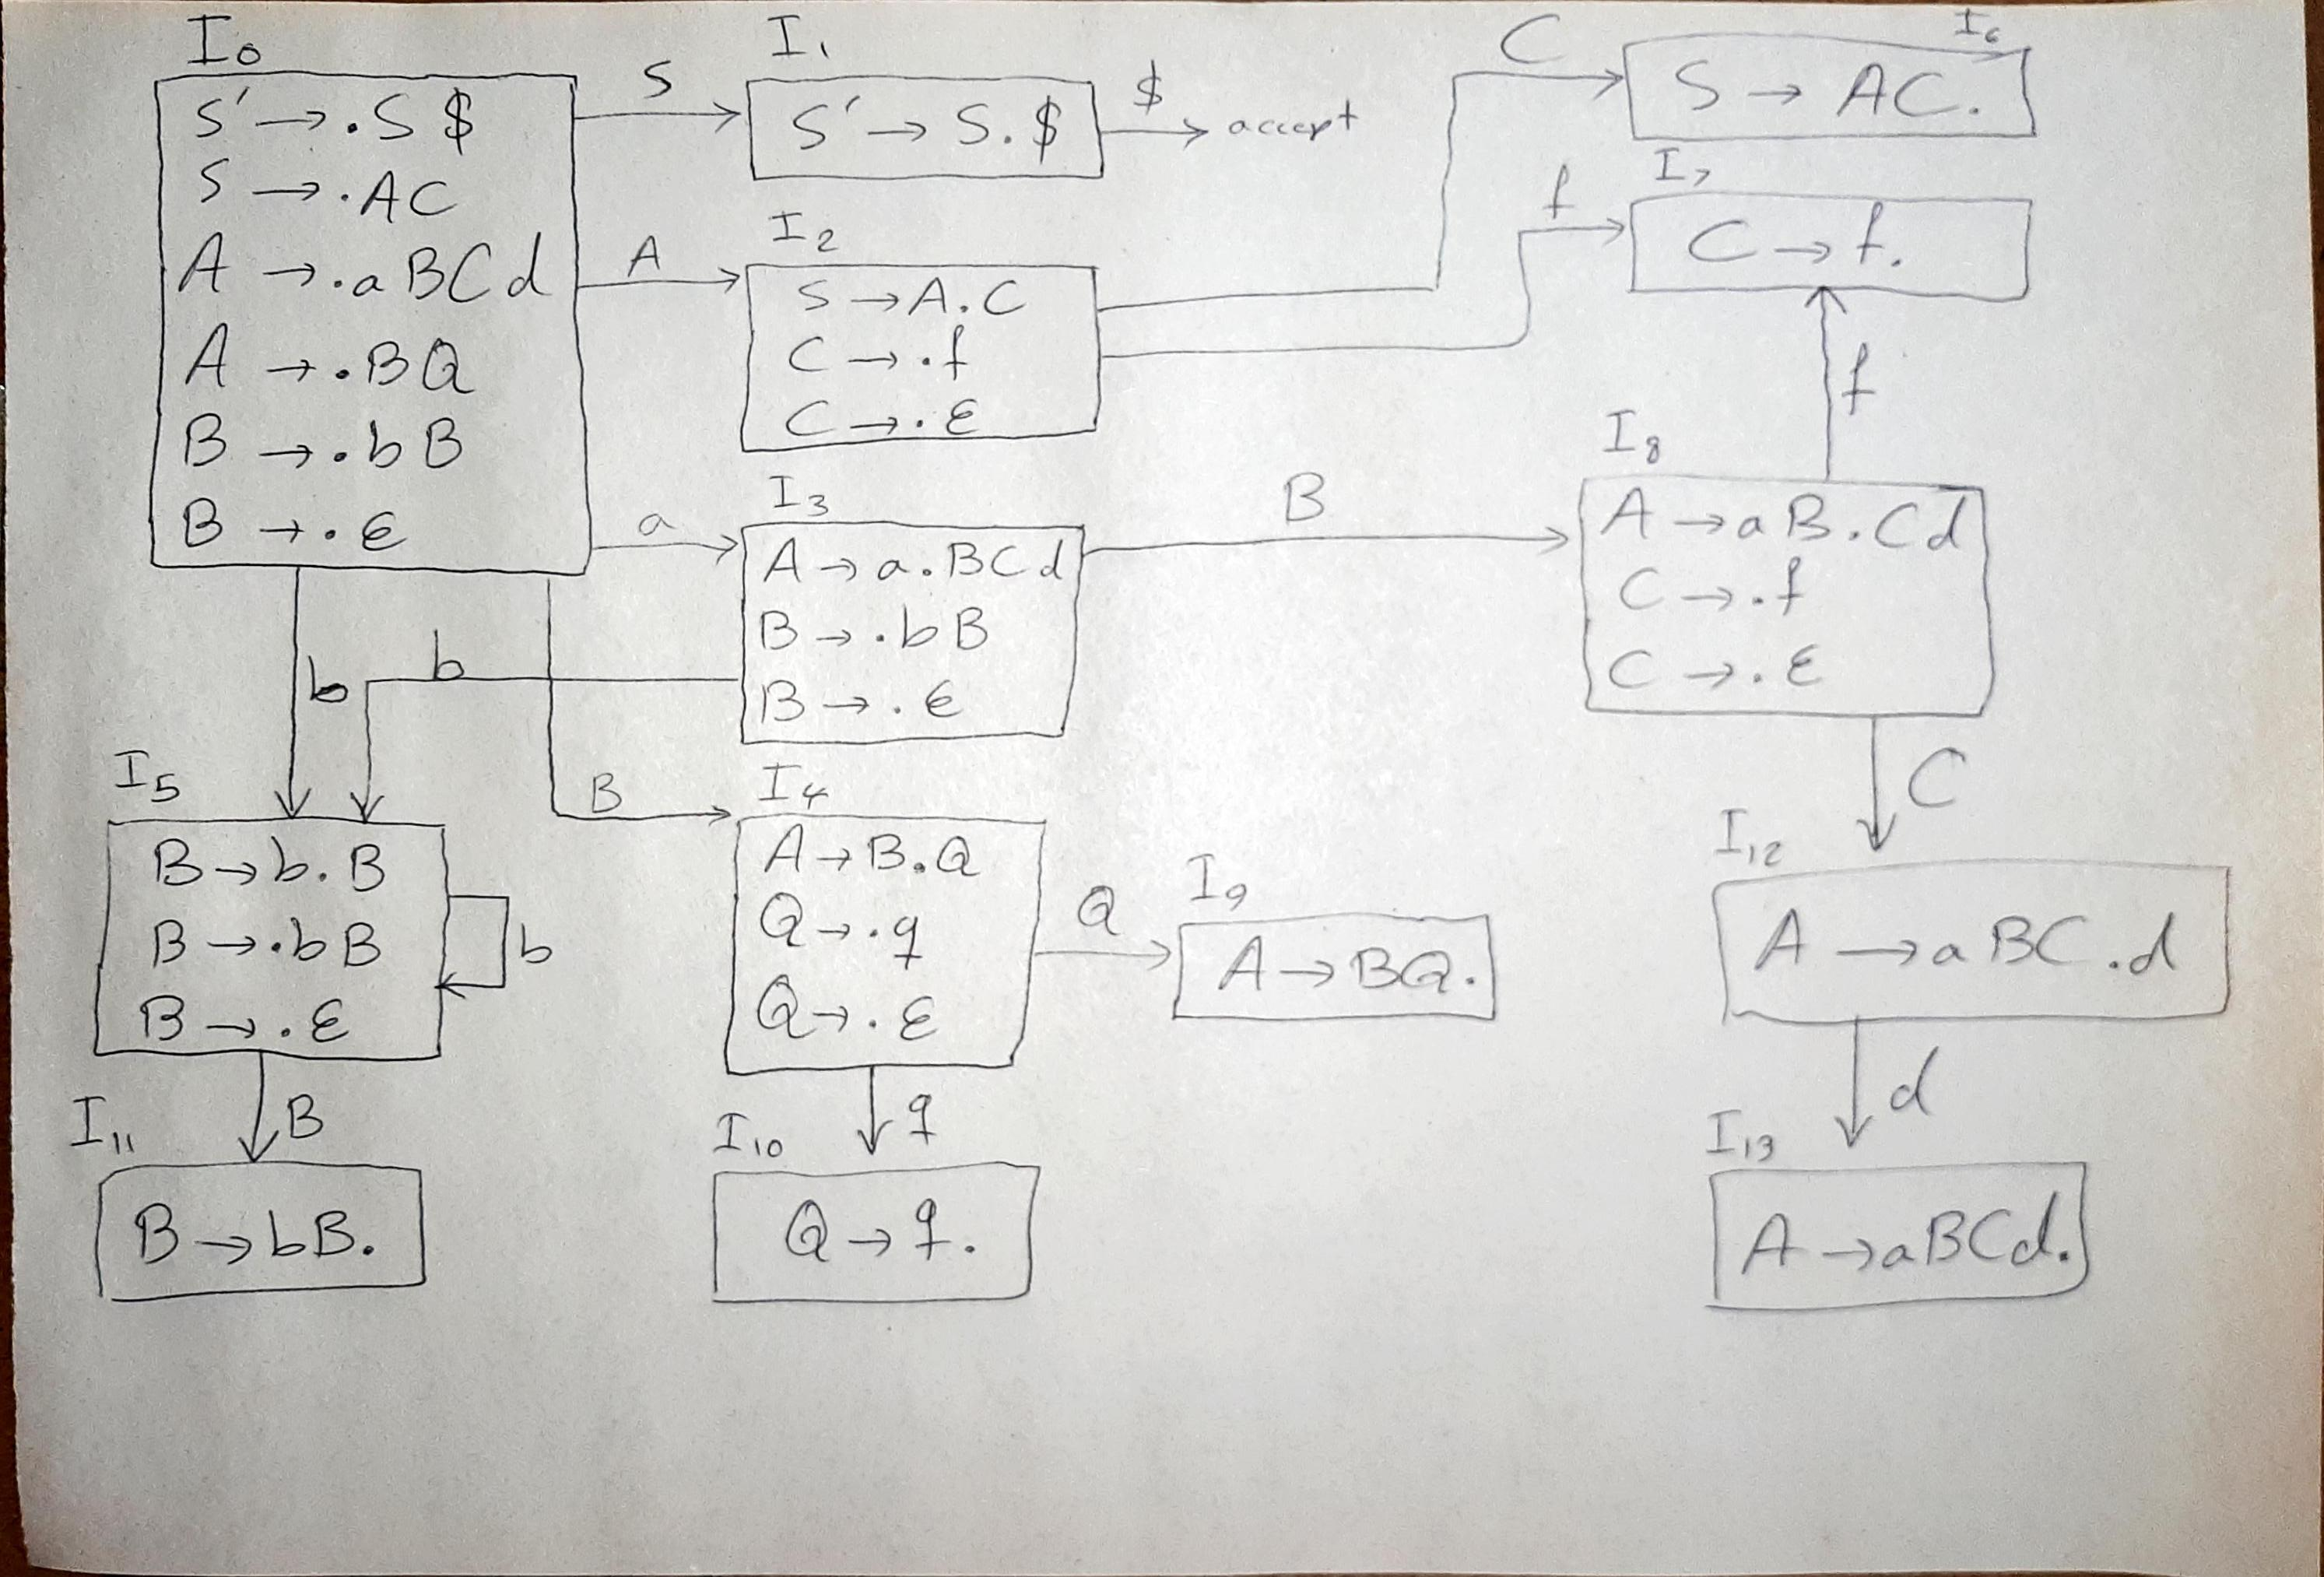
\includegraphics[width=1.0\textwidth]{figures/5.jpg}
    \caption
	{}
    \label{fig:fig1}
\end{figure}

\subsubsection{جدول تجزیه}
\begin{latin}
% Please add the following required packages to your document preamble:
% \usepackage{multirow}
% \usepackage[table,xcdraw]{xcolor}
% If you use beamer only pass "xcolor=table" option, i.e. \documentclass[xcolor=table]{beamer}
\begin{table}[H]
\begin{tabular}{|ccccccccccccc|}
\hline
\multicolumn{13}{|c|}{\textbf{LR table}}                                                                                                                                                                                                                                                                                                                                                                                                                                                                                                           \\ \hline
\multicolumn{1}{|c|}{}                                 & \multicolumn{6}{c|}{\textbf{ACTION}}                                                                                                                                                                                      & \multicolumn{6}{c|}{\textbf{GOTO}}                                                                                                                                                                                                                            \\ \cline{2-13} 
\multicolumn{1}{|c|}{\multirow{-2}{*}{\textbf{State}}} & \multicolumn{1}{c|}{\textbf{a}} & \multicolumn{1}{c|}{\textbf{d}} & \multicolumn{1}{c|}{\textbf{b}} & \multicolumn{1}{c|}{\textbf{f}} & \multicolumn{1}{c|}{\textbf{q}} & \multicolumn{1}{c|}{\textbf{\$}}                & \multicolumn{1}{c|}{\textbf{S'}} & \multicolumn{1}{c|}{\textbf{S}}               & \multicolumn{1}{c|}{\textbf{A}}               & \multicolumn{1}{c|}{\textbf{B}}                & \multicolumn{1}{c|}{\textbf{C}}                & \textbf{Q}               \\ \hline
\multicolumn{1}{|c|}{{\color[HTML]{0000FF} 0}}         & \multicolumn{1}{c|}{s3}         & \multicolumn{1}{c|}{r5}         & \multicolumn{1}{c|}{s5}         & \multicolumn{1}{c|}{r5}         & \multicolumn{1}{c|}{r5}         & \multicolumn{1}{c|}{r5}                         & \multicolumn{1}{c|}{}            & \multicolumn{1}{c|}{{\color[HTML]{0000FF} 1}} & \multicolumn{1}{c|}{{\color[HTML]{0000FF} 2}} & \multicolumn{1}{c|}{{\color[HTML]{0000FF} 4}}  & \multicolumn{1}{c|}{}                          &                          \\ \hline
\multicolumn{1}{|c|}{{\color[HTML]{0000FF} 1}}         & \multicolumn{1}{c|}{}           & \multicolumn{1}{c|}{}           & \multicolumn{1}{c|}{}           & \multicolumn{1}{c|}{}           & \multicolumn{1}{c|}{}           & \multicolumn{1}{c|}{{\color[HTML]{008000} acc}} & \multicolumn{1}{c|}{}            & \multicolumn{1}{c|}{}                         & \multicolumn{1}{c|}{}                         & \multicolumn{1}{c|}{}                          & \multicolumn{1}{c|}{}                          &                          \\ \hline
\multicolumn{1}{|c|}{{\color[HTML]{0000FF} 2}}         & \multicolumn{1}{c|}{}           & \multicolumn{1}{c|}{r7}         & \multicolumn{1}{c|}{}           & \multicolumn{1}{c|}{s7}         & \multicolumn{1}{c|}{}           & \multicolumn{1}{c|}{r7}                         & \multicolumn{1}{c|}{}            & \multicolumn{1}{c|}{}                         & \multicolumn{1}{c|}{}                         & \multicolumn{1}{c|}{}                          & \multicolumn{1}{c|}{{\color[HTML]{0000FF} 6}}  &                          \\ \hline
\multicolumn{1}{|c|}{{\color[HTML]{0000FF} 3}}         & \multicolumn{1}{c|}{}           & \multicolumn{1}{c|}{r5}         & \multicolumn{1}{c|}{s5}         & \multicolumn{1}{c|}{r5}         & \multicolumn{1}{c|}{r5}         & \multicolumn{1}{c|}{r5}                         & \multicolumn{1}{c|}{}            & \multicolumn{1}{c|}{}                         & \multicolumn{1}{c|}{}                         & \multicolumn{1}{c|}{{\color[HTML]{0000FF} 8}}  & \multicolumn{1}{c|}{}                          &                          \\ \hline
\multicolumn{1}{|c|}{{\color[HTML]{0000FF} 4}}         & \multicolumn{1}{c|}{}           & \multicolumn{1}{c|}{}           & \multicolumn{1}{c|}{}           & \multicolumn{1}{c|}{r9}         & \multicolumn{1}{c|}{s10}        & \multicolumn{1}{c|}{r9}                         & \multicolumn{1}{c|}{}            & \multicolumn{1}{c|}{}                         & \multicolumn{1}{c|}{}                         & \multicolumn{1}{c|}{}                          & \multicolumn{1}{c|}{}                          & {\color[HTML]{0000FF} 9} \\ \hline
\multicolumn{1}{|c|}{{\color[HTML]{0000FF} 5}}         & \multicolumn{1}{c|}{}           & \multicolumn{1}{c|}{r5}         & \multicolumn{1}{c|}{s5}         & \multicolumn{1}{c|}{r5}         & \multicolumn{1}{c|}{r5}         & \multicolumn{1}{c|}{r5}                         & \multicolumn{1}{c|}{}            & \multicolumn{1}{c|}{}                         & \multicolumn{1}{c|}{}                         & \multicolumn{1}{c|}{{\color[HTML]{0000FF} 11}} & \multicolumn{1}{c|}{}                          &                          \\ \hline
\multicolumn{1}{|c|}{{\color[HTML]{0000FF} 6}}         & \multicolumn{1}{c|}{}           & \multicolumn{1}{c|}{}           & \multicolumn{1}{c|}{}           & \multicolumn{1}{c|}{}           & \multicolumn{1}{c|}{}           & \multicolumn{1}{c|}{r1}                         & \multicolumn{1}{c|}{}            & \multicolumn{1}{c|}{}                         & \multicolumn{1}{c|}{}                         & \multicolumn{1}{c|}{}                          & \multicolumn{1}{c|}{}                          &                          \\ \hline
\multicolumn{1}{|c|}{{\color[HTML]{0000FF} 7}}         & \multicolumn{1}{c|}{}           & \multicolumn{1}{c|}{r6}         & \multicolumn{1}{c|}{}           & \multicolumn{1}{c|}{}           & \multicolumn{1}{c|}{}           & \multicolumn{1}{c|}{r6}                         & \multicolumn{1}{c|}{}            & \multicolumn{1}{c|}{}                         & \multicolumn{1}{c|}{}                         & \multicolumn{1}{c|}{}                          & \multicolumn{1}{c|}{}                          &                          \\ \hline
\multicolumn{1}{|c|}{{\color[HTML]{0000FF} 8}}         & \multicolumn{1}{c|}{}           & \multicolumn{1}{c|}{r7}         & \multicolumn{1}{c|}{}           & \multicolumn{1}{c|}{s7}         & \multicolumn{1}{c|}{}           & \multicolumn{1}{c|}{r7}                         & \multicolumn{1}{c|}{}            & \multicolumn{1}{c|}{}                         & \multicolumn{1}{c|}{}                         & \multicolumn{1}{c|}{}                          & \multicolumn{1}{c|}{{\color[HTML]{0000FF} 12}} &                          \\ \hline
\multicolumn{1}{|c|}{{\color[HTML]{0000FF} 9}}         & \multicolumn{1}{c|}{}           & \multicolumn{1}{c|}{}           & \multicolumn{1}{c|}{}           & \multicolumn{1}{c|}{r3}         & \multicolumn{1}{c|}{}           & \multicolumn{1}{c|}{r3}                         & \multicolumn{1}{c|}{}            & \multicolumn{1}{c|}{}                         & \multicolumn{1}{c|}{}                         & \multicolumn{1}{c|}{}                          & \multicolumn{1}{c|}{}                          &                          \\ \hline
\multicolumn{1}{|c|}{{\color[HTML]{0000FF} 10}}        & \multicolumn{1}{c|}{}           & \multicolumn{1}{c|}{}           & \multicolumn{1}{c|}{}           & \multicolumn{1}{c|}{r8}         & \multicolumn{1}{c|}{}           & \multicolumn{1}{c|}{r8}                         & \multicolumn{1}{c|}{}            & \multicolumn{1}{c|}{}                         & \multicolumn{1}{c|}{}                         & \multicolumn{1}{c|}{}                          & \multicolumn{1}{c|}{}                          &                          \\ \hline
\multicolumn{1}{|c|}{{\color[HTML]{0000FF} 11}}        & \multicolumn{1}{c|}{}           & \multicolumn{1}{c|}{r4}         & \multicolumn{1}{c|}{}           & \multicolumn{1}{c|}{r4}         & \multicolumn{1}{c|}{r4}         & \multicolumn{1}{c|}{r4}                         & \multicolumn{1}{c|}{}            & \multicolumn{1}{c|}{}                         & \multicolumn{1}{c|}{}                         & \multicolumn{1}{c|}{}                          & \multicolumn{1}{c|}{}                          &                          \\ \hline
\multicolumn{1}{|c|}{{\color[HTML]{0000FF} 12}}        & \multicolumn{1}{c|}{}           & \multicolumn{1}{c|}{s13}        & \multicolumn{1}{c|}{}           & \multicolumn{1}{c|}{}           & \multicolumn{1}{c|}{}           & \multicolumn{1}{c|}{}                           & \multicolumn{1}{c|}{}            & \multicolumn{1}{c|}{}                         & \multicolumn{1}{c|}{}                         & \multicolumn{1}{c|}{}                          & \multicolumn{1}{c|}{}                          &                          \\ \hline
\multicolumn{1}{|c|}{{\color[HTML]{0000FF} 13}}        & \multicolumn{1}{c|}{}           & \multicolumn{1}{c|}{}           & \multicolumn{1}{c|}{}           & \multicolumn{1}{c|}{r2}         & \multicolumn{1}{c|}{}           & \multicolumn{1}{c|}{r2}                         & \multicolumn{1}{c|}{}            & \multicolumn{1}{c|}{}                         & \multicolumn{1}{c|}{}                         & \multicolumn{1}{c|}{}                          & \multicolumn{1}{c|}{}                          &                          \\ \hline
\end{tabular}
\end{table}
\end{latin}


\subsection{}
\begin{latin}
% Please add the following required packages to your document preamble:
% \usepackage[table,xcdraw]{xcolor}
% If you use beamer only pass "xcolor=table" option, i.e. \documentclass[xcolor=table]{beamer}
\begin{table}[H]
\begin{tabular}{|llll|}
\hline
\multicolumn{4}{|c|}{\textbf{Trace}}                                                                                                                                               \\ \hline
\multicolumn{1}{|c|}{\textbf{Step}} & \multicolumn{1}{c|}{\textbf{Stack}}                             & \multicolumn{1}{c|}{\textbf{Input}} & \multicolumn{1}{c|}{\textbf{Action}} \\ \hline
\multicolumn{1}{|l|}{1}             & \multicolumn{1}{l|}{{\color[HTML]{0000FF} 0}}                   & \multicolumn{1}{l|}{a b b d f \$}   & s3                                   \\ \hline
\multicolumn{1}{|l|}{2}             & \multicolumn{1}{l|}{{\color[HTML]{0000FF} 0 a 3}}               & \multicolumn{1}{l|}{b b d f \$}     & s5                                   \\ \hline
\multicolumn{1}{|l|}{3}             & \multicolumn{1}{l|}{{\color[HTML]{0000FF} 0 a 3 b 5}}           & \multicolumn{1}{l|}{b d f \$}       & s5                                   \\ \hline
\multicolumn{1}{|l|}{4}             & \multicolumn{1}{l|}{{\color[HTML]{0000FF} 0 a 3 b 5 b 5}}       & \multicolumn{1}{l|}{d f \$}         & r5                                   \\ \hline
\multicolumn{1}{|l|}{5}             & \multicolumn{1}{l|}{{\color[HTML]{0000FF} 0 a 3 b 5 b 5 B}}     & \multicolumn{1}{l|}{d f \$}         & {\color[HTML]{0000FF} 11}            \\ \hline
\multicolumn{1}{|l|}{6}             & \multicolumn{1}{l|}{{\color[HTML]{0000FF} 0 a 3 b 5 b 5 B 11}}  & \multicolumn{1}{l|}{d f \$}         & r4                                   \\ \hline
\multicolumn{1}{|l|}{7}             & \multicolumn{1}{l|}{{\color[HTML]{0000FF} 0 a 3 b 5 B}}         & \multicolumn{1}{l|}{d f \$}         & {\color[HTML]{0000FF} 11}            \\ \hline
\multicolumn{1}{|l|}{8}             & \multicolumn{1}{l|}{{\color[HTML]{0000FF} 0 a 3 b 5 B 11}}      & \multicolumn{1}{l|}{d f \$}         & r4                                   \\ \hline
\multicolumn{1}{|l|}{9}             & \multicolumn{1}{l|}{{\color[HTML]{0000FF} 0 a 3 B}}             & \multicolumn{1}{l|}{d f \$}         & {\color[HTML]{0000FF} 8}             \\ \hline
\multicolumn{1}{|l|}{10}            & \multicolumn{1}{l|}{{\color[HTML]{0000FF} 0 a 3 B 8}}           & \multicolumn{1}{l|}{d f \$}         & r7                                   \\ \hline
\multicolumn{1}{|l|}{11}            & \multicolumn{1}{l|}{{\color[HTML]{0000FF} 0 a 3 B 8 C}}         & \multicolumn{1}{l|}{d f \$}         & {\color[HTML]{0000FF} 12}            \\ \hline
\multicolumn{1}{|l|}{12}            & \multicolumn{1}{l|}{{\color[HTML]{0000FF} 0 a 3 B 8 C 12}}      & \multicolumn{1}{l|}{d f \$}         & s13                                  \\ \hline
\multicolumn{1}{|l|}{13}            & \multicolumn{1}{l|}{{\color[HTML]{0000FF} 0 a 3 B 8 C 12 d 13}} & \multicolumn{1}{l|}{f \$}           & r2                                   \\ \hline
\multicolumn{1}{|l|}{14}            & \multicolumn{1}{l|}{{\color[HTML]{0000FF} 0 A}}                 & \multicolumn{1}{l|}{f \$}           & {\color[HTML]{0000FF} 2}             \\ \hline
\multicolumn{1}{|l|}{15}            & \multicolumn{1}{l|}{{\color[HTML]{0000FF} 0 A 2}}               & \multicolumn{1}{l|}{f \$}           & s7                                   \\ \hline
\multicolumn{1}{|l|}{16}            & \multicolumn{1}{l|}{{\color[HTML]{0000FF} 0 A 2 f 7}}           & \multicolumn{1}{l|}{\$}             & r6                                   \\ \hline
\multicolumn{1}{|l|}{17}            & \multicolumn{1}{l|}{{\color[HTML]{0000FF} 0 A 2 C}}             & \multicolumn{1}{l|}{\$}             & {\color[HTML]{0000FF} 6}             \\ \hline
\multicolumn{1}{|l|}{18}            & \multicolumn{1}{l|}{{\color[HTML]{0000FF} 0 A 2 C 6}}           & \multicolumn{1}{l|}{\$}             & r1                                   \\ \hline
\multicolumn{1}{|l|}{19}            & \multicolumn{1}{l|}{{\color[HTML]{0000FF} 0 S}}                 & \multicolumn{1}{l|}{\$}             & {\color[HTML]{0000FF} 1}             \\ \hline
\multicolumn{1}{|l|}{20}            & \multicolumn{1}{l|}{{\color[HTML]{0000FF} 0 S 1}}               & \multicolumn{1}{l|}{\$}             & {\color[HTML]{008000} acc}           \\ \hline
\end{tabular}
\end{table}
\end{latin}



\section{}%6
\subsection{آ}
\begin{figure}[H]
    \centering
    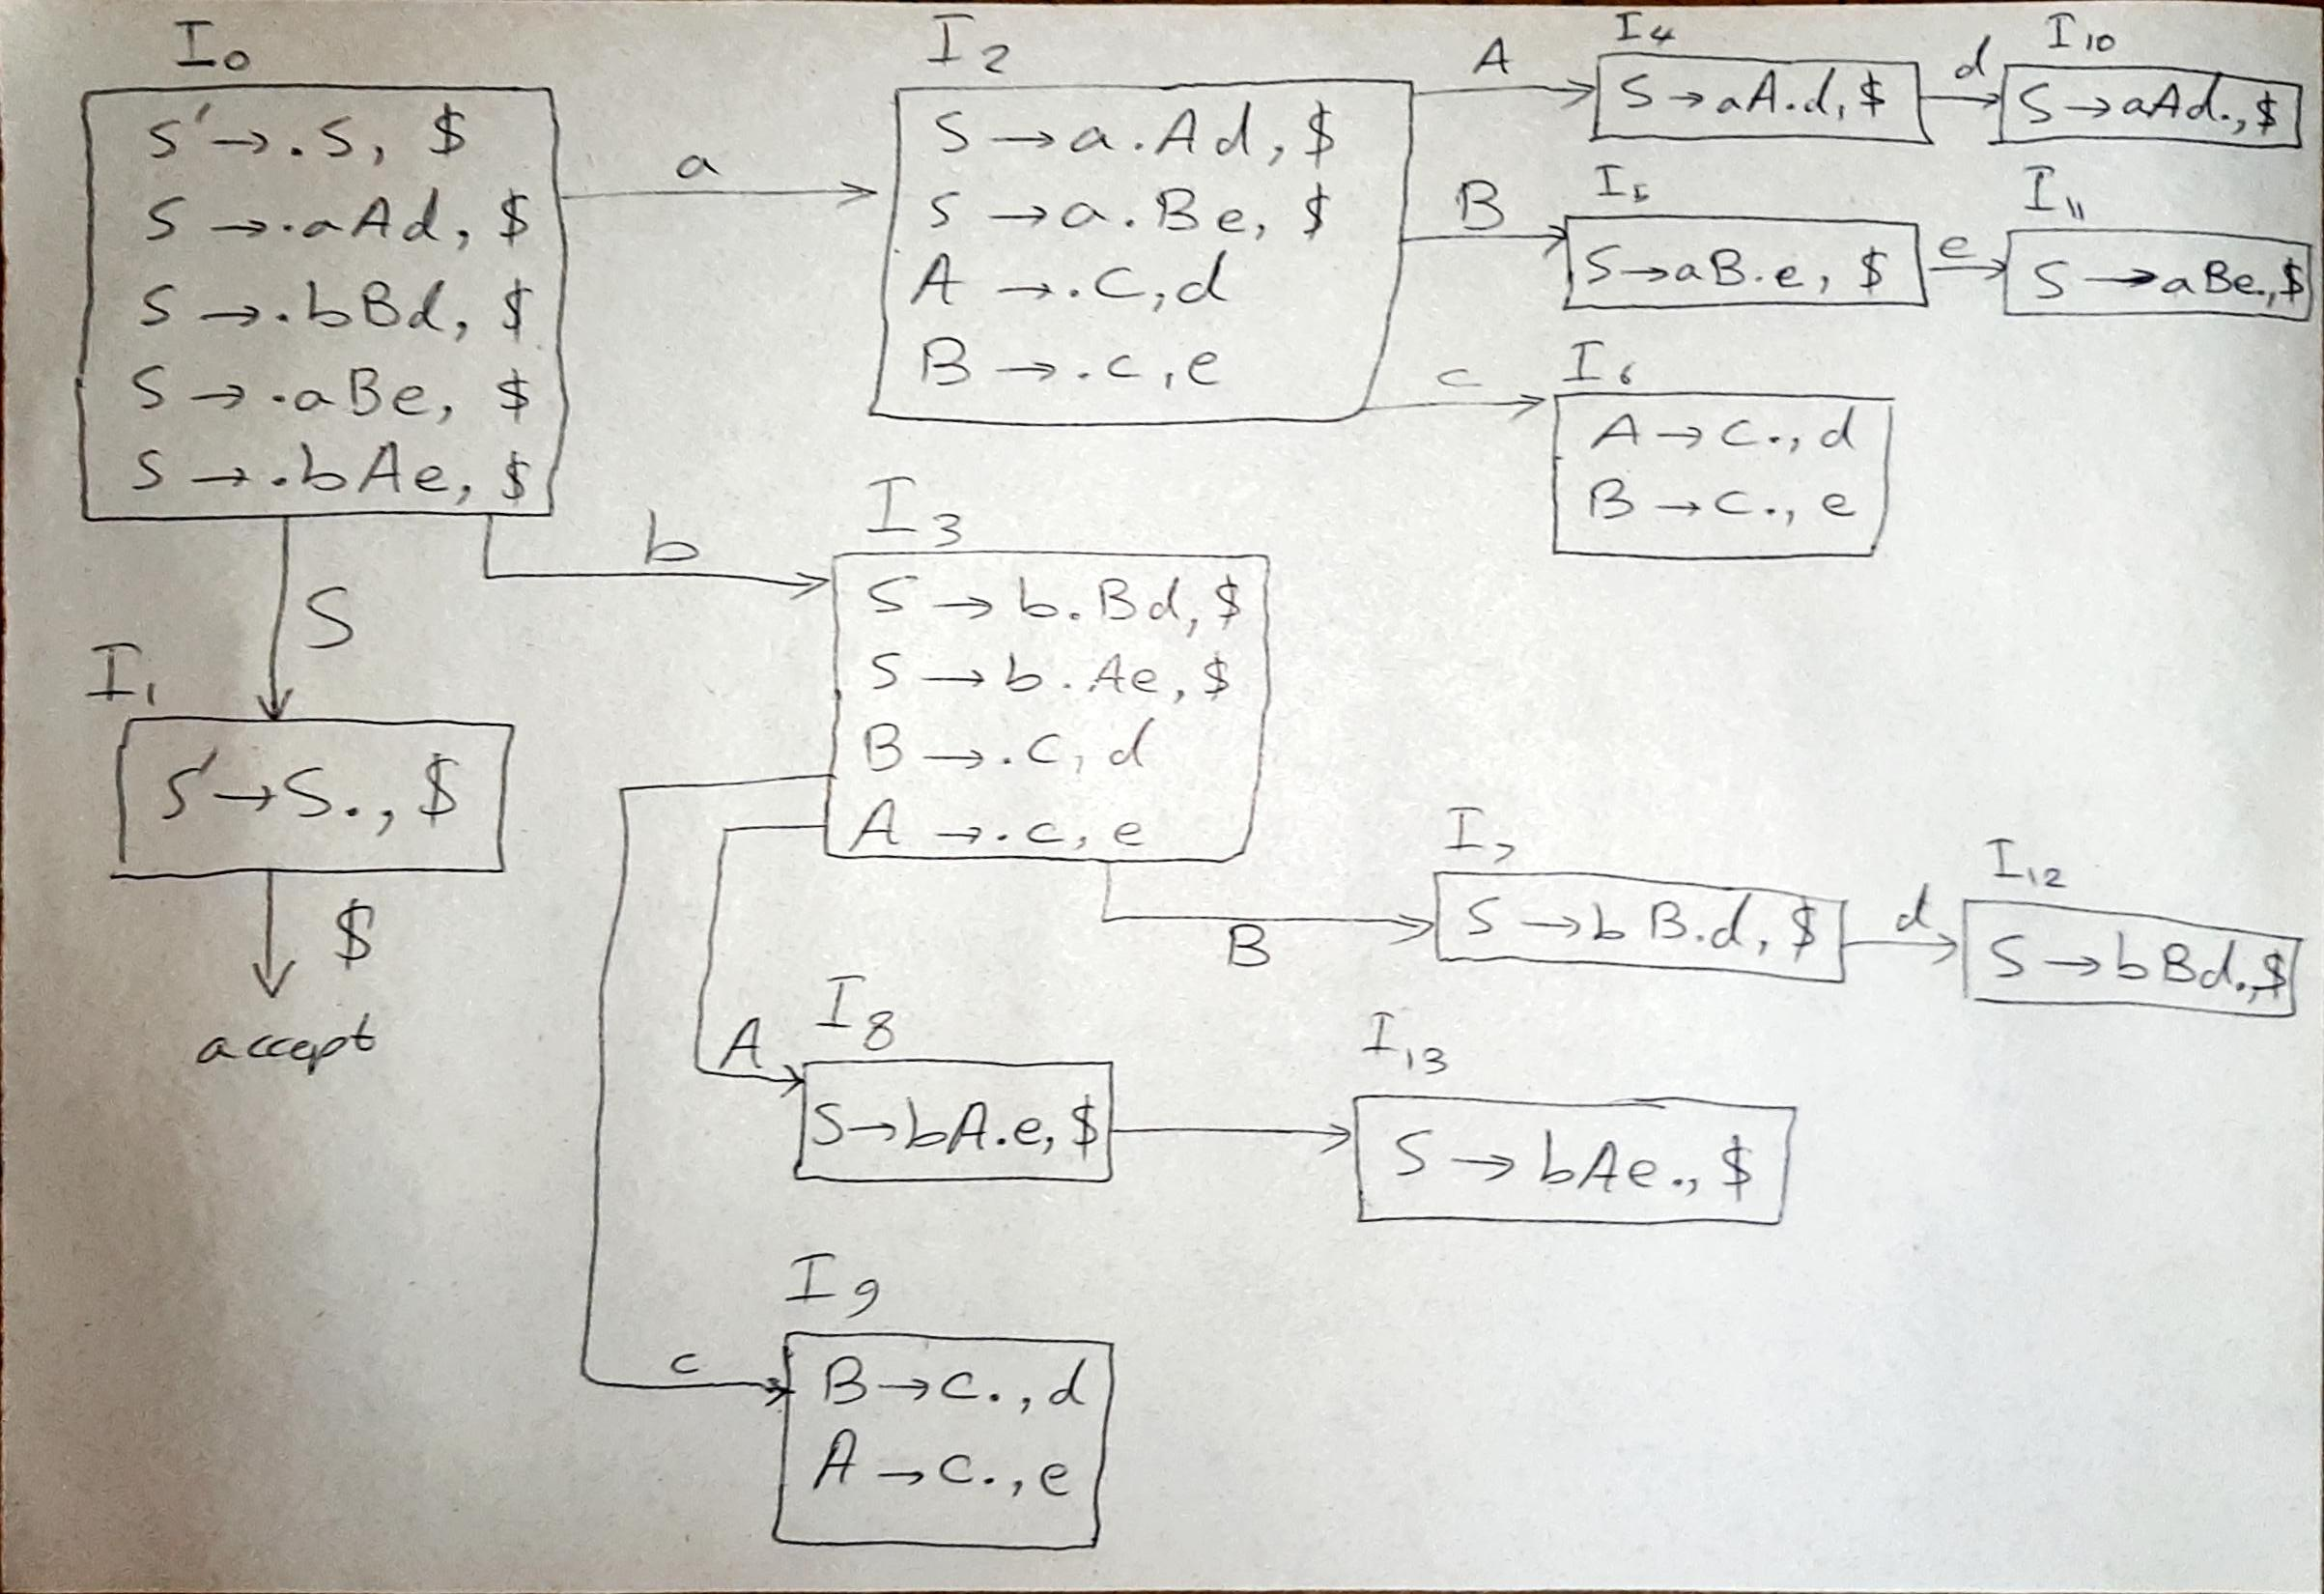
\includegraphics[width=1.0\textwidth]{figures/6.jpg}
    \caption
	{}
    \label{fig:fig1}
\end{figure}

\subsection{ب}
\begin{latin}
% Please add the following required packages to your document preamble:
% \usepackage{multirow}
% \usepackage[table,xcdraw]{xcolor}
% If you use beamer only pass "xcolor=table" option, i.e. \documentclass[xcolor=table]{beamer}
\begin{table}[H]
\begin{tabular}{|ccccccccccc|}
\hline
\multicolumn{11}{|c|}{\textbf{LR table}}                                                                                                                                                                                                                                                                                                                                                                                                         \\ \hline
\multicolumn{1}{|c|}{}                                 & \multicolumn{6}{c|}{\textbf{ACTION}}                                                                                                                                                                                      & \multicolumn{4}{c|}{\textbf{GOTO}}                                                                                                                          \\ \cline{2-11} 
\multicolumn{1}{|c|}{\multirow{-2}{*}{\textbf{State}}} & \multicolumn{1}{c|}{\textbf{a}} & \multicolumn{1}{c|}{\textbf{d}} & \multicolumn{1}{c|}{\textbf{b}} & \multicolumn{1}{c|}{\textbf{e}} & \multicolumn{1}{c|}{\textbf{c}} & \multicolumn{1}{c|}{\textbf{\$}}                & \multicolumn{1}{c|}{\textbf{S'}} & \multicolumn{1}{c|}{\textbf{S}}               & \multicolumn{1}{c|}{\textbf{A}}               & \textbf{B}               \\ \hline
\multicolumn{1}{|c|}{{\color[HTML]{0000FF} 0}}         & \multicolumn{1}{c|}{s2}         & \multicolumn{1}{c|}{}           & \multicolumn{1}{c|}{s3}         & \multicolumn{1}{c|}{}           & \multicolumn{1}{c|}{}           & \multicolumn{1}{c|}{}                           & \multicolumn{1}{c|}{}            & \multicolumn{1}{c|}{{\color[HTML]{0000FF} 1}} & \multicolumn{1}{c|}{}                         &                          \\ \hline
\multicolumn{1}{|c|}{{\color[HTML]{0000FF} 1}}         & \multicolumn{1}{c|}{}           & \multicolumn{1}{c|}{}           & \multicolumn{1}{c|}{}           & \multicolumn{1}{c|}{}           & \multicolumn{1}{c|}{}           & \multicolumn{1}{c|}{{\color[HTML]{008000} acc}} & \multicolumn{1}{c|}{}            & \multicolumn{1}{c|}{}                         & \multicolumn{1}{c|}{}                         &                          \\ \hline
\multicolumn{1}{|c|}{{\color[HTML]{0000FF} 2}}         & \multicolumn{1}{c|}{}           & \multicolumn{1}{c|}{}           & \multicolumn{1}{c|}{}           & \multicolumn{1}{c|}{}           & \multicolumn{1}{c|}{s6}         & \multicolumn{1}{c|}{}                           & \multicolumn{1}{c|}{}            & \multicolumn{1}{c|}{}                         & \multicolumn{1}{c|}{{\color[HTML]{0000FF} 4}} & {\color[HTML]{0000FF} 5} \\ \hline
\multicolumn{1}{|c|}{{\color[HTML]{0000FF} 3}}         & \multicolumn{1}{c|}{}           & \multicolumn{1}{c|}{}           & \multicolumn{1}{c|}{}           & \multicolumn{1}{c|}{}           & \multicolumn{1}{c|}{s9}         & \multicolumn{1}{c|}{}                           & \multicolumn{1}{c|}{}            & \multicolumn{1}{c|}{}                         & \multicolumn{1}{c|}{{\color[HTML]{0000FF} 8}} & {\color[HTML]{0000FF} 7} \\ \hline
\multicolumn{1}{|c|}{{\color[HTML]{0000FF} 4}}         & \multicolumn{1}{c|}{}           & \multicolumn{1}{c|}{s10}        & \multicolumn{1}{c|}{}           & \multicolumn{1}{c|}{}           & \multicolumn{1}{c|}{}           & \multicolumn{1}{c|}{}                           & \multicolumn{1}{c|}{}            & \multicolumn{1}{c|}{}                         & \multicolumn{1}{c|}{}                         &                          \\ \hline
\multicolumn{1}{|c|}{{\color[HTML]{0000FF} 5}}         & \multicolumn{1}{c|}{}           & \multicolumn{1}{c|}{}           & \multicolumn{1}{c|}{}           & \multicolumn{1}{c|}{s11}        & \multicolumn{1}{c|}{}           & \multicolumn{1}{c|}{}                           & \multicolumn{1}{c|}{}            & \multicolumn{1}{c|}{}                         & \multicolumn{1}{c|}{}                         &                          \\ \hline
\multicolumn{1}{|c|}{{\color[HTML]{0000FF} 6}}         & \multicolumn{1}{c|}{}           & \multicolumn{1}{c|}{r5}         & \multicolumn{1}{c|}{}           & \multicolumn{1}{c|}{r6}         & \multicolumn{1}{c|}{}           & \multicolumn{1}{c|}{}                           & \multicolumn{1}{c|}{}            & \multicolumn{1}{c|}{}                         & \multicolumn{1}{c|}{}                         &                          \\ \hline
\multicolumn{1}{|c|}{{\color[HTML]{0000FF} 7}}         & \multicolumn{1}{c|}{}           & \multicolumn{1}{c|}{s12}        & \multicolumn{1}{c|}{}           & \multicolumn{1}{c|}{}           & \multicolumn{1}{c|}{}           & \multicolumn{1}{c|}{}                           & \multicolumn{1}{c|}{}            & \multicolumn{1}{c|}{}                         & \multicolumn{1}{c|}{}                         &                          \\ \hline
\multicolumn{1}{|c|}{{\color[HTML]{0000FF} 8}}         & \multicolumn{1}{c|}{}           & \multicolumn{1}{c|}{}           & \multicolumn{1}{c|}{}           & \multicolumn{1}{c|}{s13}        & \multicolumn{1}{c|}{}           & \multicolumn{1}{c|}{}                           & \multicolumn{1}{c|}{}            & \multicolumn{1}{c|}{}                         & \multicolumn{1}{c|}{}                         &                          \\ \hline
\multicolumn{1}{|c|}{{\color[HTML]{0000FF} 9}}         & \multicolumn{1}{c|}{}           & \multicolumn{1}{c|}{r6}         & \multicolumn{1}{c|}{}           & \multicolumn{1}{c|}{r5}         & \multicolumn{1}{c|}{}           & \multicolumn{1}{c|}{}                           & \multicolumn{1}{c|}{}            & \multicolumn{1}{c|}{}                         & \multicolumn{1}{c|}{}                         &                          \\ \hline
\multicolumn{1}{|c|}{{\color[HTML]{0000FF} 10}}        & \multicolumn{1}{c|}{}           & \multicolumn{1}{c|}{}           & \multicolumn{1}{c|}{}           & \multicolumn{1}{c|}{}           & \multicolumn{1}{c|}{}           & \multicolumn{1}{c|}{r1}                         & \multicolumn{1}{c|}{}            & \multicolumn{1}{c|}{}                         & \multicolumn{1}{c|}{}                         &                          \\ \hline
\multicolumn{1}{|c|}{{\color[HTML]{0000FF} 11}}        & \multicolumn{1}{c|}{}           & \multicolumn{1}{c|}{}           & \multicolumn{1}{c|}{}           & \multicolumn{1}{c|}{}           & \multicolumn{1}{c|}{}           & \multicolumn{1}{c|}{r3}                         & \multicolumn{1}{c|}{}            & \multicolumn{1}{c|}{}                         & \multicolumn{1}{c|}{}                         &                          \\ \hline
\multicolumn{1}{|c|}{{\color[HTML]{0000FF} 12}}        & \multicolumn{1}{c|}{}           & \multicolumn{1}{c|}{}           & \multicolumn{1}{c|}{}           & \multicolumn{1}{c|}{}           & \multicolumn{1}{c|}{}           & \multicolumn{1}{c|}{r2}                         & \multicolumn{1}{c|}{}            & \multicolumn{1}{c|}{}                         & \multicolumn{1}{c|}{}                         &                          \\ \hline
\multicolumn{1}{|c|}{{\color[HTML]{0000FF} 13}}        & \multicolumn{1}{c|}{}           & \multicolumn{1}{c|}{}           & \multicolumn{1}{c|}{}           & \multicolumn{1}{c|}{}           & \multicolumn{1}{c|}{}           & \multicolumn{1}{c|}{r4}                         & \multicolumn{1}{c|}{}            & \multicolumn{1}{c|}{}                         & \multicolumn{1}{c|}{}                         &                          \\ \hline
\end{tabular}
\end{table}
\end{latin}

\subsection{ج}
استیت‌های 6 و 9 باید ادغام شوند.

\subsection{د}
خیر- چون برای سمبل‌های \lr{d} و \lr{e} کانفلیکتِ \lr{reduce-reduce}ِ  \lr{r5} و \lr{r6} وجود دارد.



\section{}%7
\subsection{آ}
\begin{latin}
$\\
S^\prime \longrightarrow S \$ \\
S \longrightarrow a S | A S \\
A \longrightarrow a
$
\end{latin}

\begin{figure}[H]
    \centering
    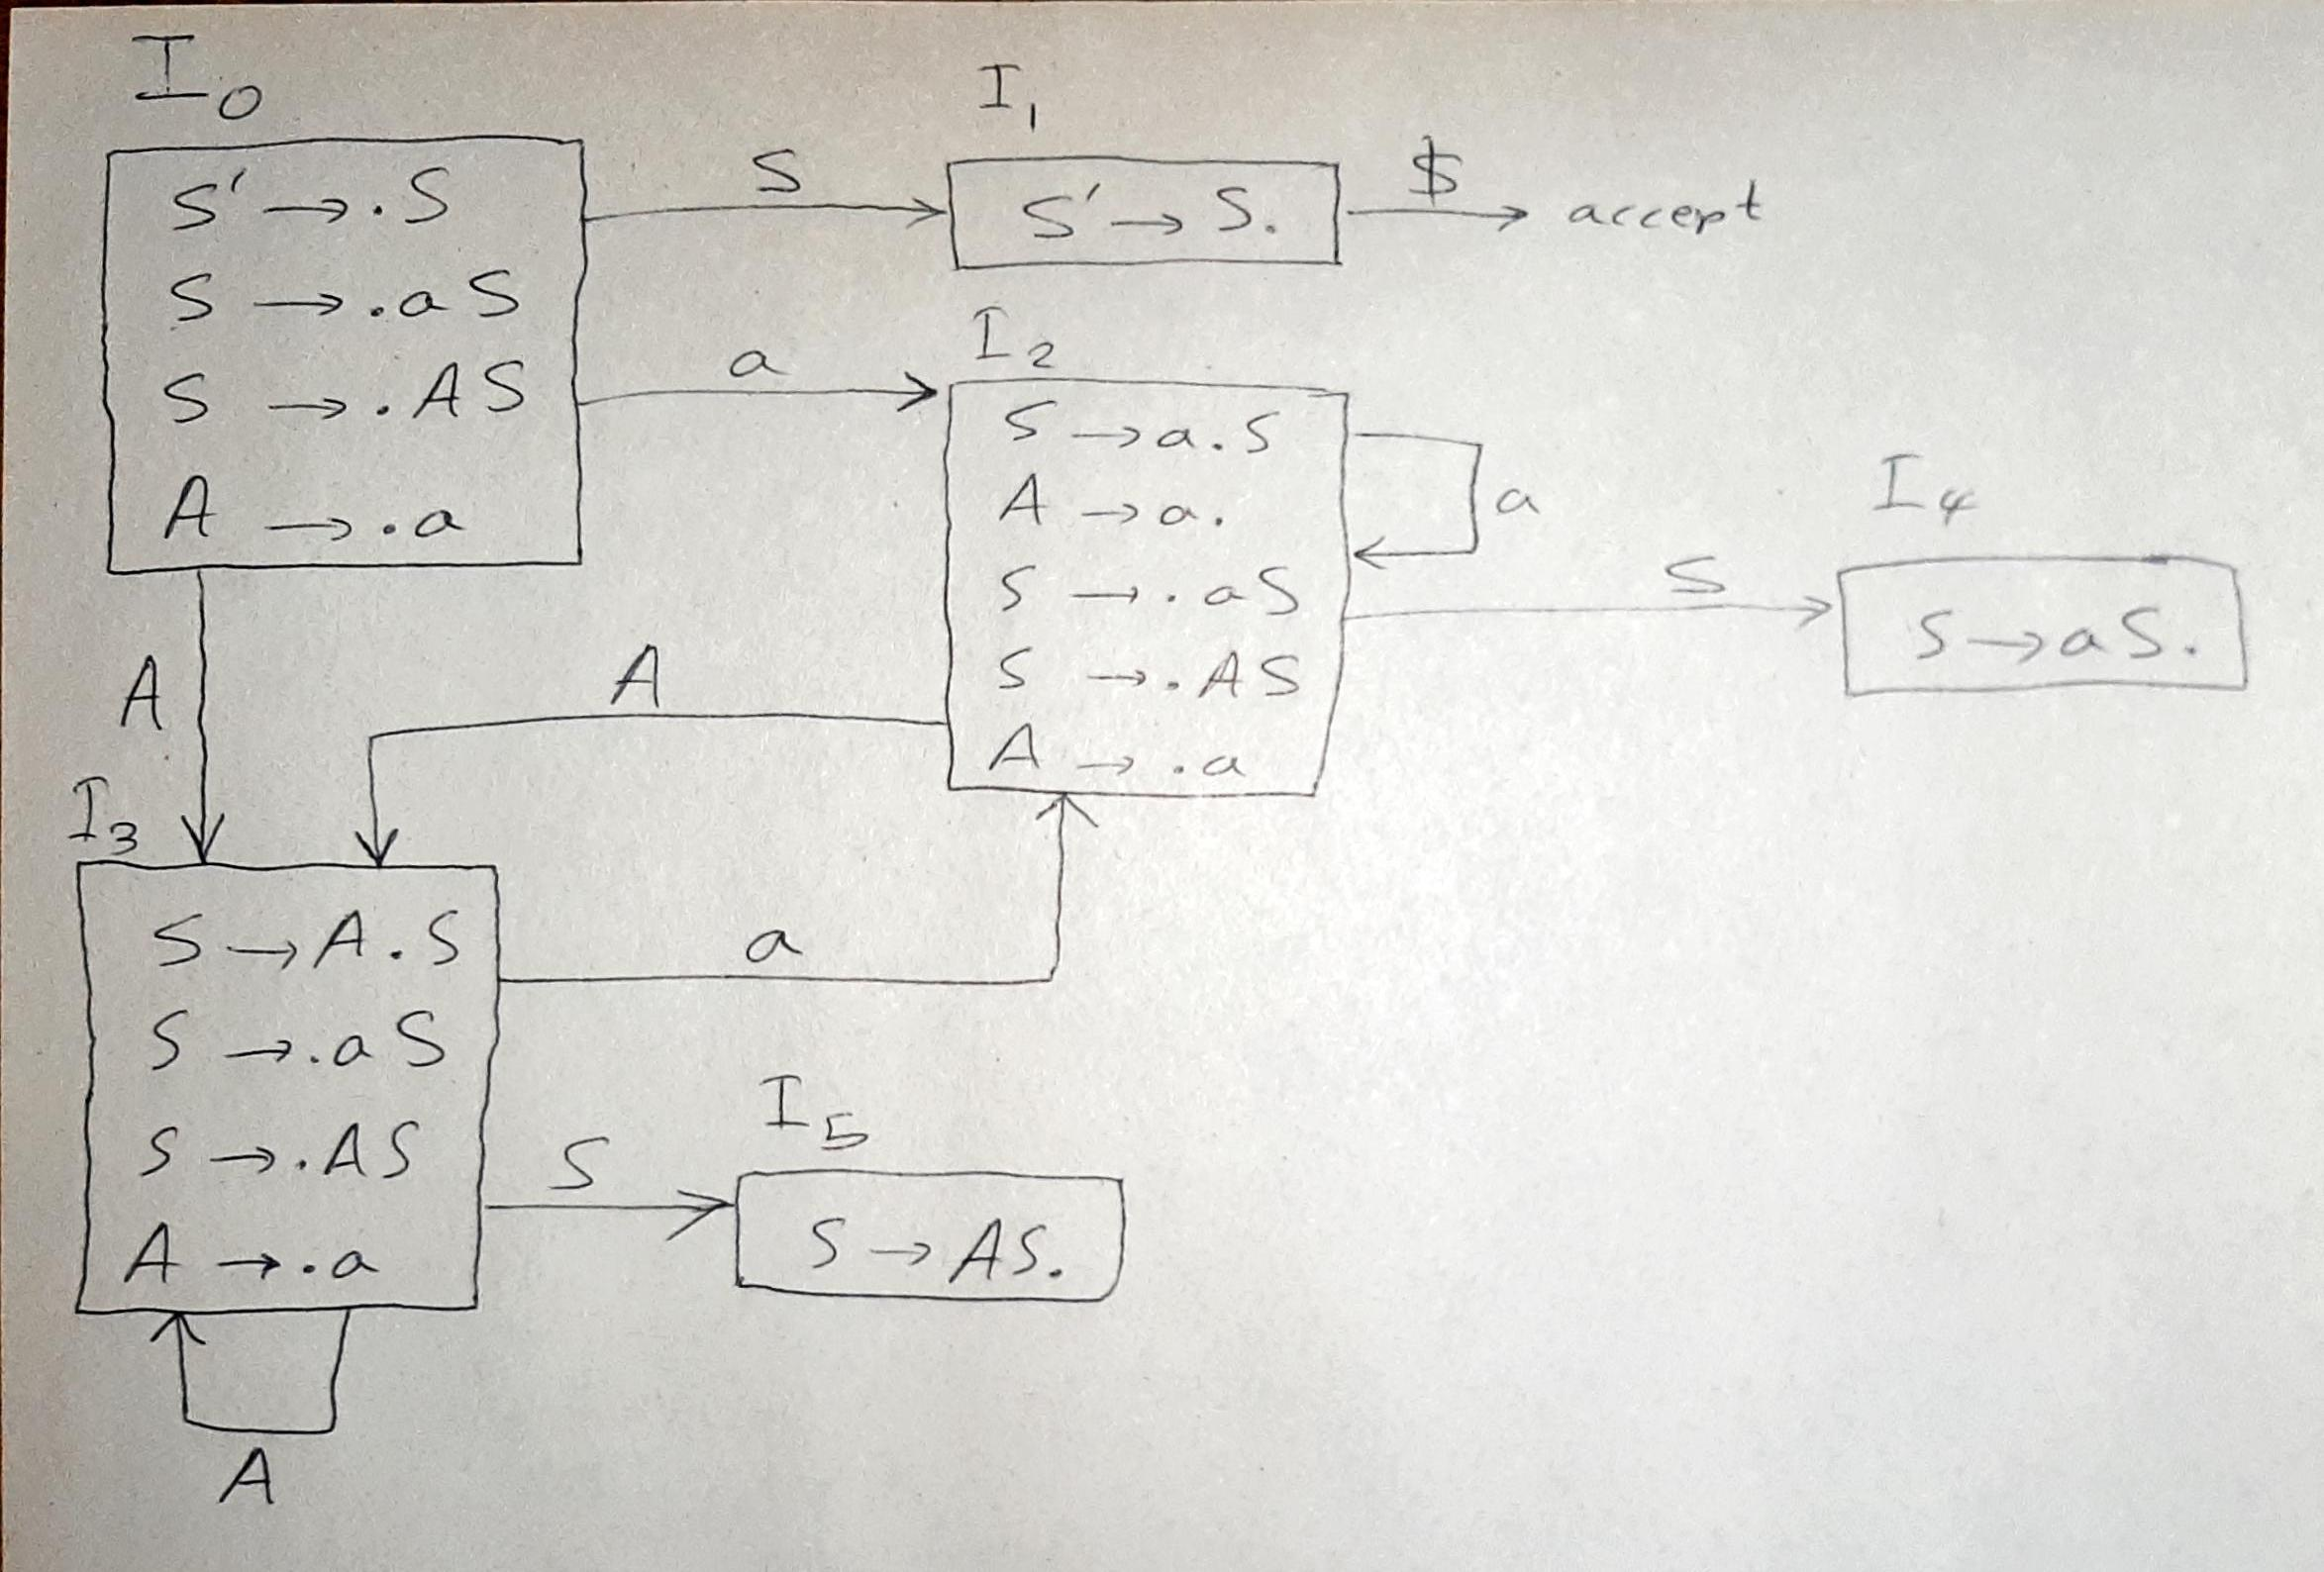
\includegraphics[width=1.0\textwidth]{figures/7a.jpg}
    \caption
	{}
    \label{fig:fig1}
\end{figure}

کانفلیکت در استیت 2.


\subsection{ب}
\begin{latin}
$\\
S^\prime \longrightarrow S \$ \\
S \longrightarrow a R | A T \\
R \longrightarrow a \\
T \longrightarrow a
$
\end{latin}

\begin{figure}[H]
    \centering
    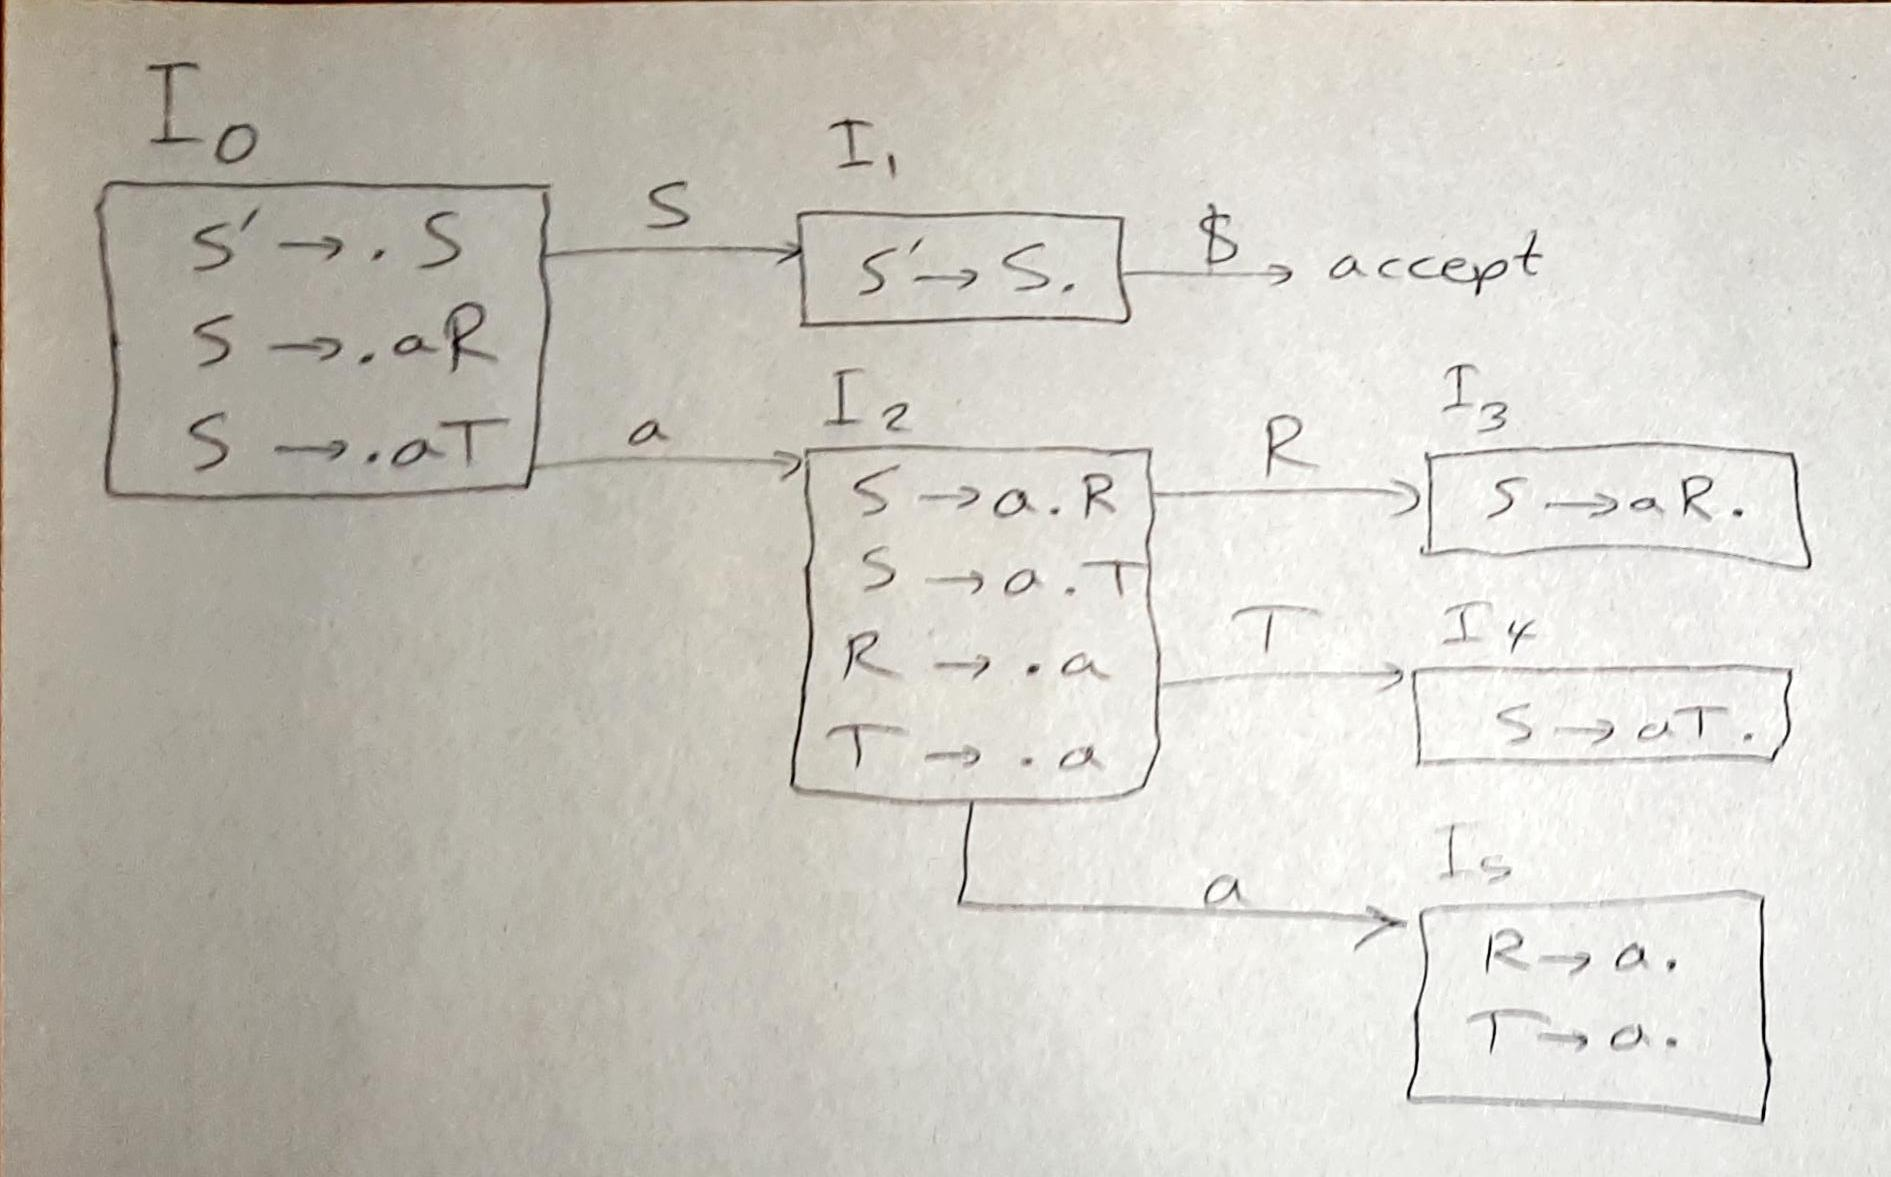
\includegraphics[width=1.0\textwidth]{figures/7b.jpg}
    \caption
	{}
    \label{fig:fig1}
\end{figure}

کانفلیکت در استیت 5.


\section{}%8
به ازای رول‌های به شکلِ
\begin{latin}
$\\
S \longrightarrow A_i b_i
$
\end{latin}
که منتج به کاهش می‌شوند هر کدام دو (نظیر حالات ممکن قرار گرفتن نقطه) آیتم $LR(0)$ داریم. پس تا اینجا حداقل $2n$ آیتم داریم.\\
به ازای رول‌های به شکلِ
\begin{latin}
$\\
A_i \longrightarrow a_j
$
\end{latin}
که منتج به کاهش می‌شوند هر کدام دو (نظیر حالات ممکن قرار گرفتن نقطه) آیتم $LR(0)$ داریم. پس $2\frac{n(n-1)}{2}$ آیتم دیگر هم داریم.\\
به ازای رول‌های به شکلِ
\begin{latin}
$\\
A_i \longrightarrow a_j A_i
$
\end{latin}
که منتج به کاهش می‌شوند $2^n$ تا آیتم داریم. پس در مجموع حداقل تعداد آیتم‌ها برابر است با:
\begin{latin}
$\\
2 ^ n + n ^ 2 + n
$
\end{latin}



\section{}%9
\subsection{آ}
جدول تجزیه‌ی $LALR(1)$ به صورت زیر است و هیچ کانفلیکتی در آن وجود ندارد.
\begin{latin}
% Please add the following required packages to your document preamble:
% \usepackage{multirow}
% \usepackage[table,xcdraw]{xcolor}
% If you use beamer only pass "xcolor=table" option, i.e. \documentclass[xcolor=table]{beamer}
\begin{table}[H]
\begin{tabular}{|ccccccccc|}
\hline
\multicolumn{9}{|c|}{\textbf{LR table}}                                                                                                                                                                                                                                                                                                                        \\ \hline
\multicolumn{1}{|c|}{}                                 & \multicolumn{5}{c|}{\textbf{ACTION}}                                                                                                                                                    & \multicolumn{3}{c|}{\textbf{GOTO}}                                                                          \\ \cline{2-9} 
\multicolumn{1}{|c|}{\multirow{-2}{*}{\textbf{State}}} & \multicolumn{1}{c|}{\textbf{a}} & \multicolumn{1}{c|}{\textbf{b}} & \multicolumn{1}{c|}{\textbf{c}} & \multicolumn{1}{c|}{\textbf{d}} & \multicolumn{1}{c|}{\textbf{\$}}                & \multicolumn{1}{c|}{\textbf{S'}} & \multicolumn{1}{c|}{\textbf{S}}               & \textbf{A}               \\ \hline
\multicolumn{1}{|c|}{{\color[HTML]{0000FF} 0}}         & \multicolumn{1}{c|}{s5}         & \multicolumn{1}{c|}{s3}         & \multicolumn{1}{c|}{}           & \multicolumn{1}{c|}{s4}         & \multicolumn{1}{c|}{}                           & \multicolumn{1}{c|}{}            & \multicolumn{1}{c|}{{\color[HTML]{0000FF} 1}} & {\color[HTML]{0000FF} 2} \\ \hline
\multicolumn{1}{|c|}{{\color[HTML]{0000FF} 1}}         & \multicolumn{1}{c|}{}           & \multicolumn{1}{c|}{}           & \multicolumn{1}{c|}{}           & \multicolumn{1}{c|}{}           & \multicolumn{1}{c|}{{\color[HTML]{008000} acc}} & \multicolumn{1}{c|}{}            & \multicolumn{1}{c|}{}                         &                          \\ \hline
\multicolumn{1}{|c|}{{\color[HTML]{0000FF} 2}}         & \multicolumn{1}{c|}{s6}         & \multicolumn{1}{c|}{}           & \multicolumn{1}{c|}{}           & \multicolumn{1}{c|}{}           & \multicolumn{1}{c|}{}                           & \multicolumn{1}{c|}{}            & \multicolumn{1}{c|}{}                         &                          \\ \hline
\multicolumn{1}{|c|}{{\color[HTML]{0000FF} 3}}         & \multicolumn{1}{c|}{s5}         & \multicolumn{1}{c|}{}           & \multicolumn{1}{c|}{}           & \multicolumn{1}{c|}{s8}         & \multicolumn{1}{c|}{}                           & \multicolumn{1}{c|}{}            & \multicolumn{1}{c|}{}                         & {\color[HTML]{0000FF} 7} \\ \hline
\multicolumn{1}{|c|}{{\color[HTML]{0000FF} 4}}         & \multicolumn{1}{c|}{r6}         & \multicolumn{1}{c|}{}           & \multicolumn{1}{c|}{s9}         & \multicolumn{1}{c|}{}           & \multicolumn{1}{c|}{}                           & \multicolumn{1}{c|}{}            & \multicolumn{1}{c|}{}                         &                          \\ \hline
\multicolumn{1}{|c|}{{\color[HTML]{0000FF} 5}}         & \multicolumn{1}{c|}{r5}         & \multicolumn{1}{c|}{}           & \multicolumn{1}{c|}{r5}         & \multicolumn{1}{c|}{}           & \multicolumn{1}{c|}{}                           & \multicolumn{1}{c|}{}            & \multicolumn{1}{c|}{}                         &                          \\ \hline
\multicolumn{1}{|c|}{{\color[HTML]{0000FF} 6}}         & \multicolumn{1}{c|}{}           & \multicolumn{1}{c|}{}           & \multicolumn{1}{c|}{}           & \multicolumn{1}{c|}{}           & \multicolumn{1}{c|}{r1}                         & \multicolumn{1}{c|}{}            & \multicolumn{1}{c|}{}                         &                          \\ \hline
\multicolumn{1}{|c|}{{\color[HTML]{0000FF} 7}}         & \multicolumn{1}{c|}{}           & \multicolumn{1}{c|}{}           & \multicolumn{1}{c|}{s10}        & \multicolumn{1}{c|}{}           & \multicolumn{1}{c|}{}                           & \multicolumn{1}{c|}{}            & \multicolumn{1}{c|}{}                         &                          \\ \hline
\multicolumn{1}{|c|}{{\color[HTML]{0000FF} 8}}         & \multicolumn{1}{c|}{s11}        & \multicolumn{1}{c|}{}           & \multicolumn{1}{c|}{r6}         & \multicolumn{1}{c|}{}           & \multicolumn{1}{c|}{}                           & \multicolumn{1}{c|}{}            & \multicolumn{1}{c|}{}                         &                          \\ \hline
\multicolumn{1}{|c|}{{\color[HTML]{0000FF} 9}}         & \multicolumn{1}{c|}{}           & \multicolumn{1}{c|}{}           & \multicolumn{1}{c|}{}           & \multicolumn{1}{c|}{}           & \multicolumn{1}{c|}{r3}                         & \multicolumn{1}{c|}{}            & \multicolumn{1}{c|}{}                         &                          \\ \hline
\multicolumn{1}{|c|}{{\color[HTML]{0000FF} 10}}        & \multicolumn{1}{c|}{}           & \multicolumn{1}{c|}{}           & \multicolumn{1}{c|}{}           & \multicolumn{1}{c|}{}           & \multicolumn{1}{c|}{r2}                         & \multicolumn{1}{c|}{}            & \multicolumn{1}{c|}{}                         &                          \\ \hline
\multicolumn{1}{|c|}{{\color[HTML]{0000FF} 11}}        & \multicolumn{1}{c|}{}           & \multicolumn{1}{c|}{}           & \multicolumn{1}{c|}{}           & \multicolumn{1}{c|}{}           & \multicolumn{1}{c|}{r4}                         & \multicolumn{1}{c|}{}            & \multicolumn{1}{c|}{}                         &                          \\ \hline
\end{tabular}
\end{table}
\end{latin}

با مشاهده‌ی بخشی از نمودار حالت $SLR(1)$ و \lr{FOLLOW}ی \lr{A} و \lr{S} که برابر با $\left\{ a, b, d \right\}$ است، می‌بینیم که یک کانفلیکتِ \lr{shift-reduce} در استیت 4 وجود دارد که نشان می‌دهد این گرامر $SLR(1)$ نیست.
\begin{figure}[H]
    \centering
    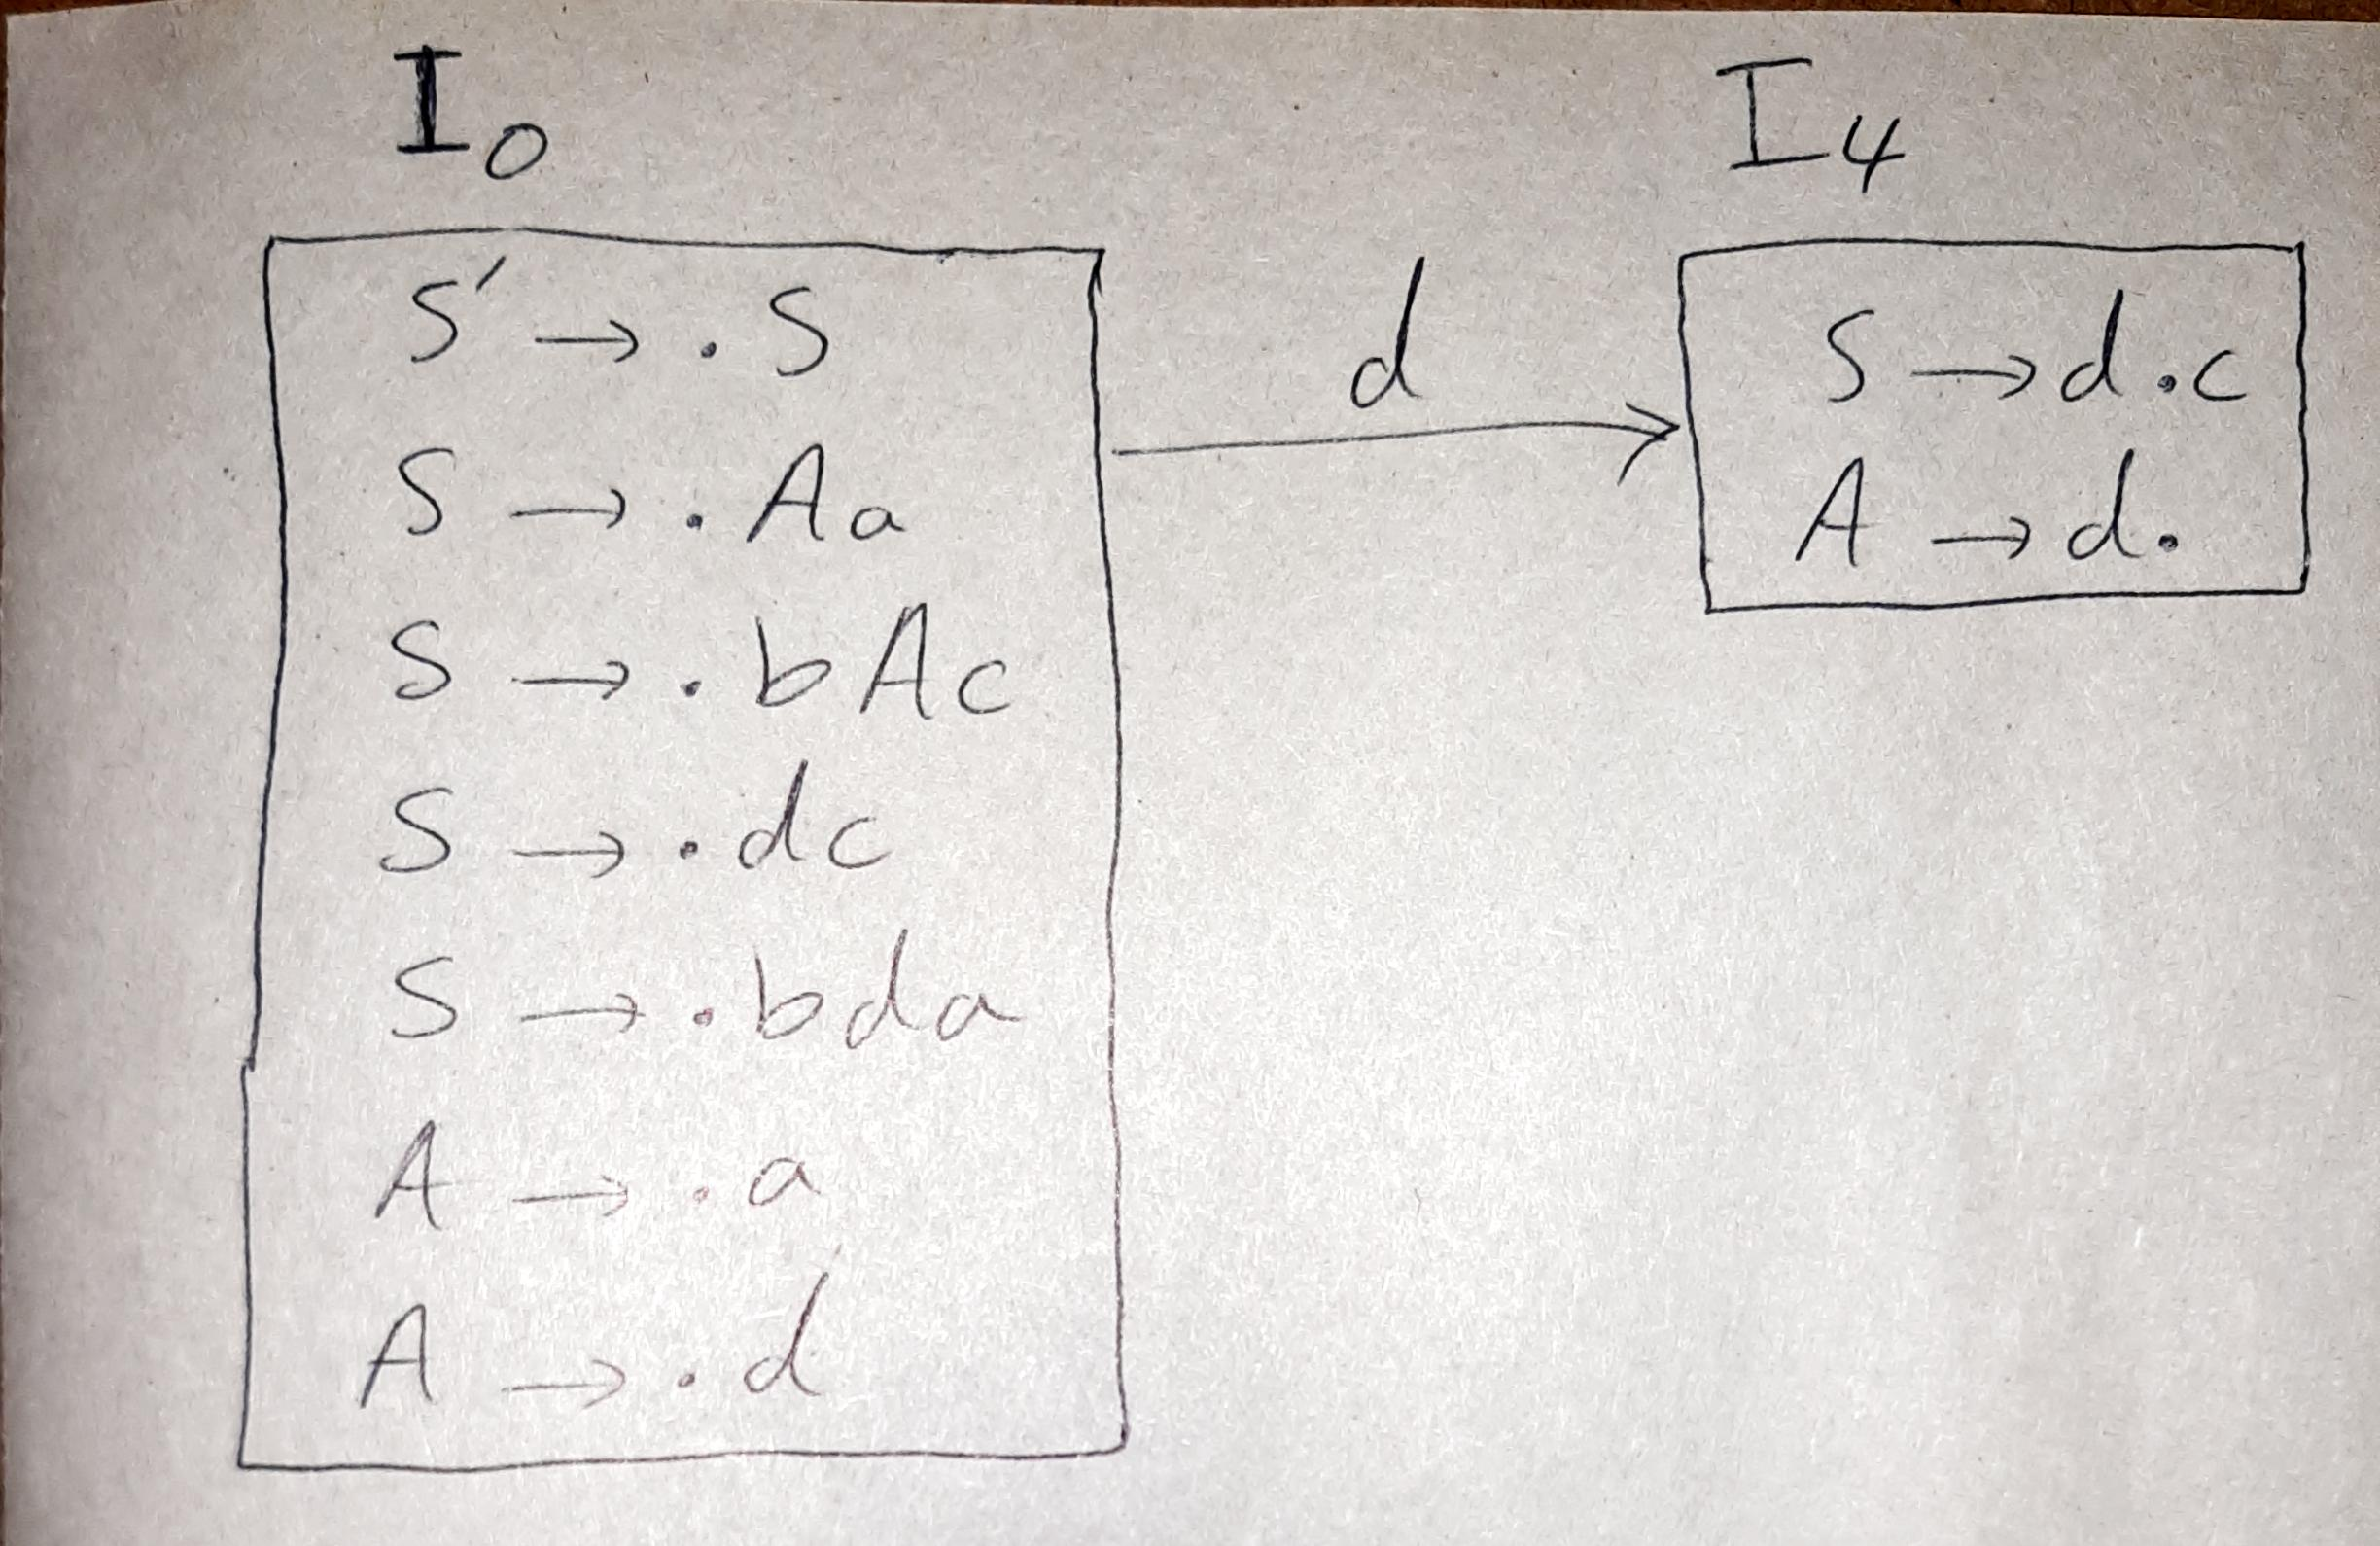
\includegraphics[width=0.75\textwidth]{figures/9a.jpg}
    \caption
	{}
    \label{fig:fig1}
\end{figure}

\subsection{ب}
\begin{figure}[H]
    \centering
    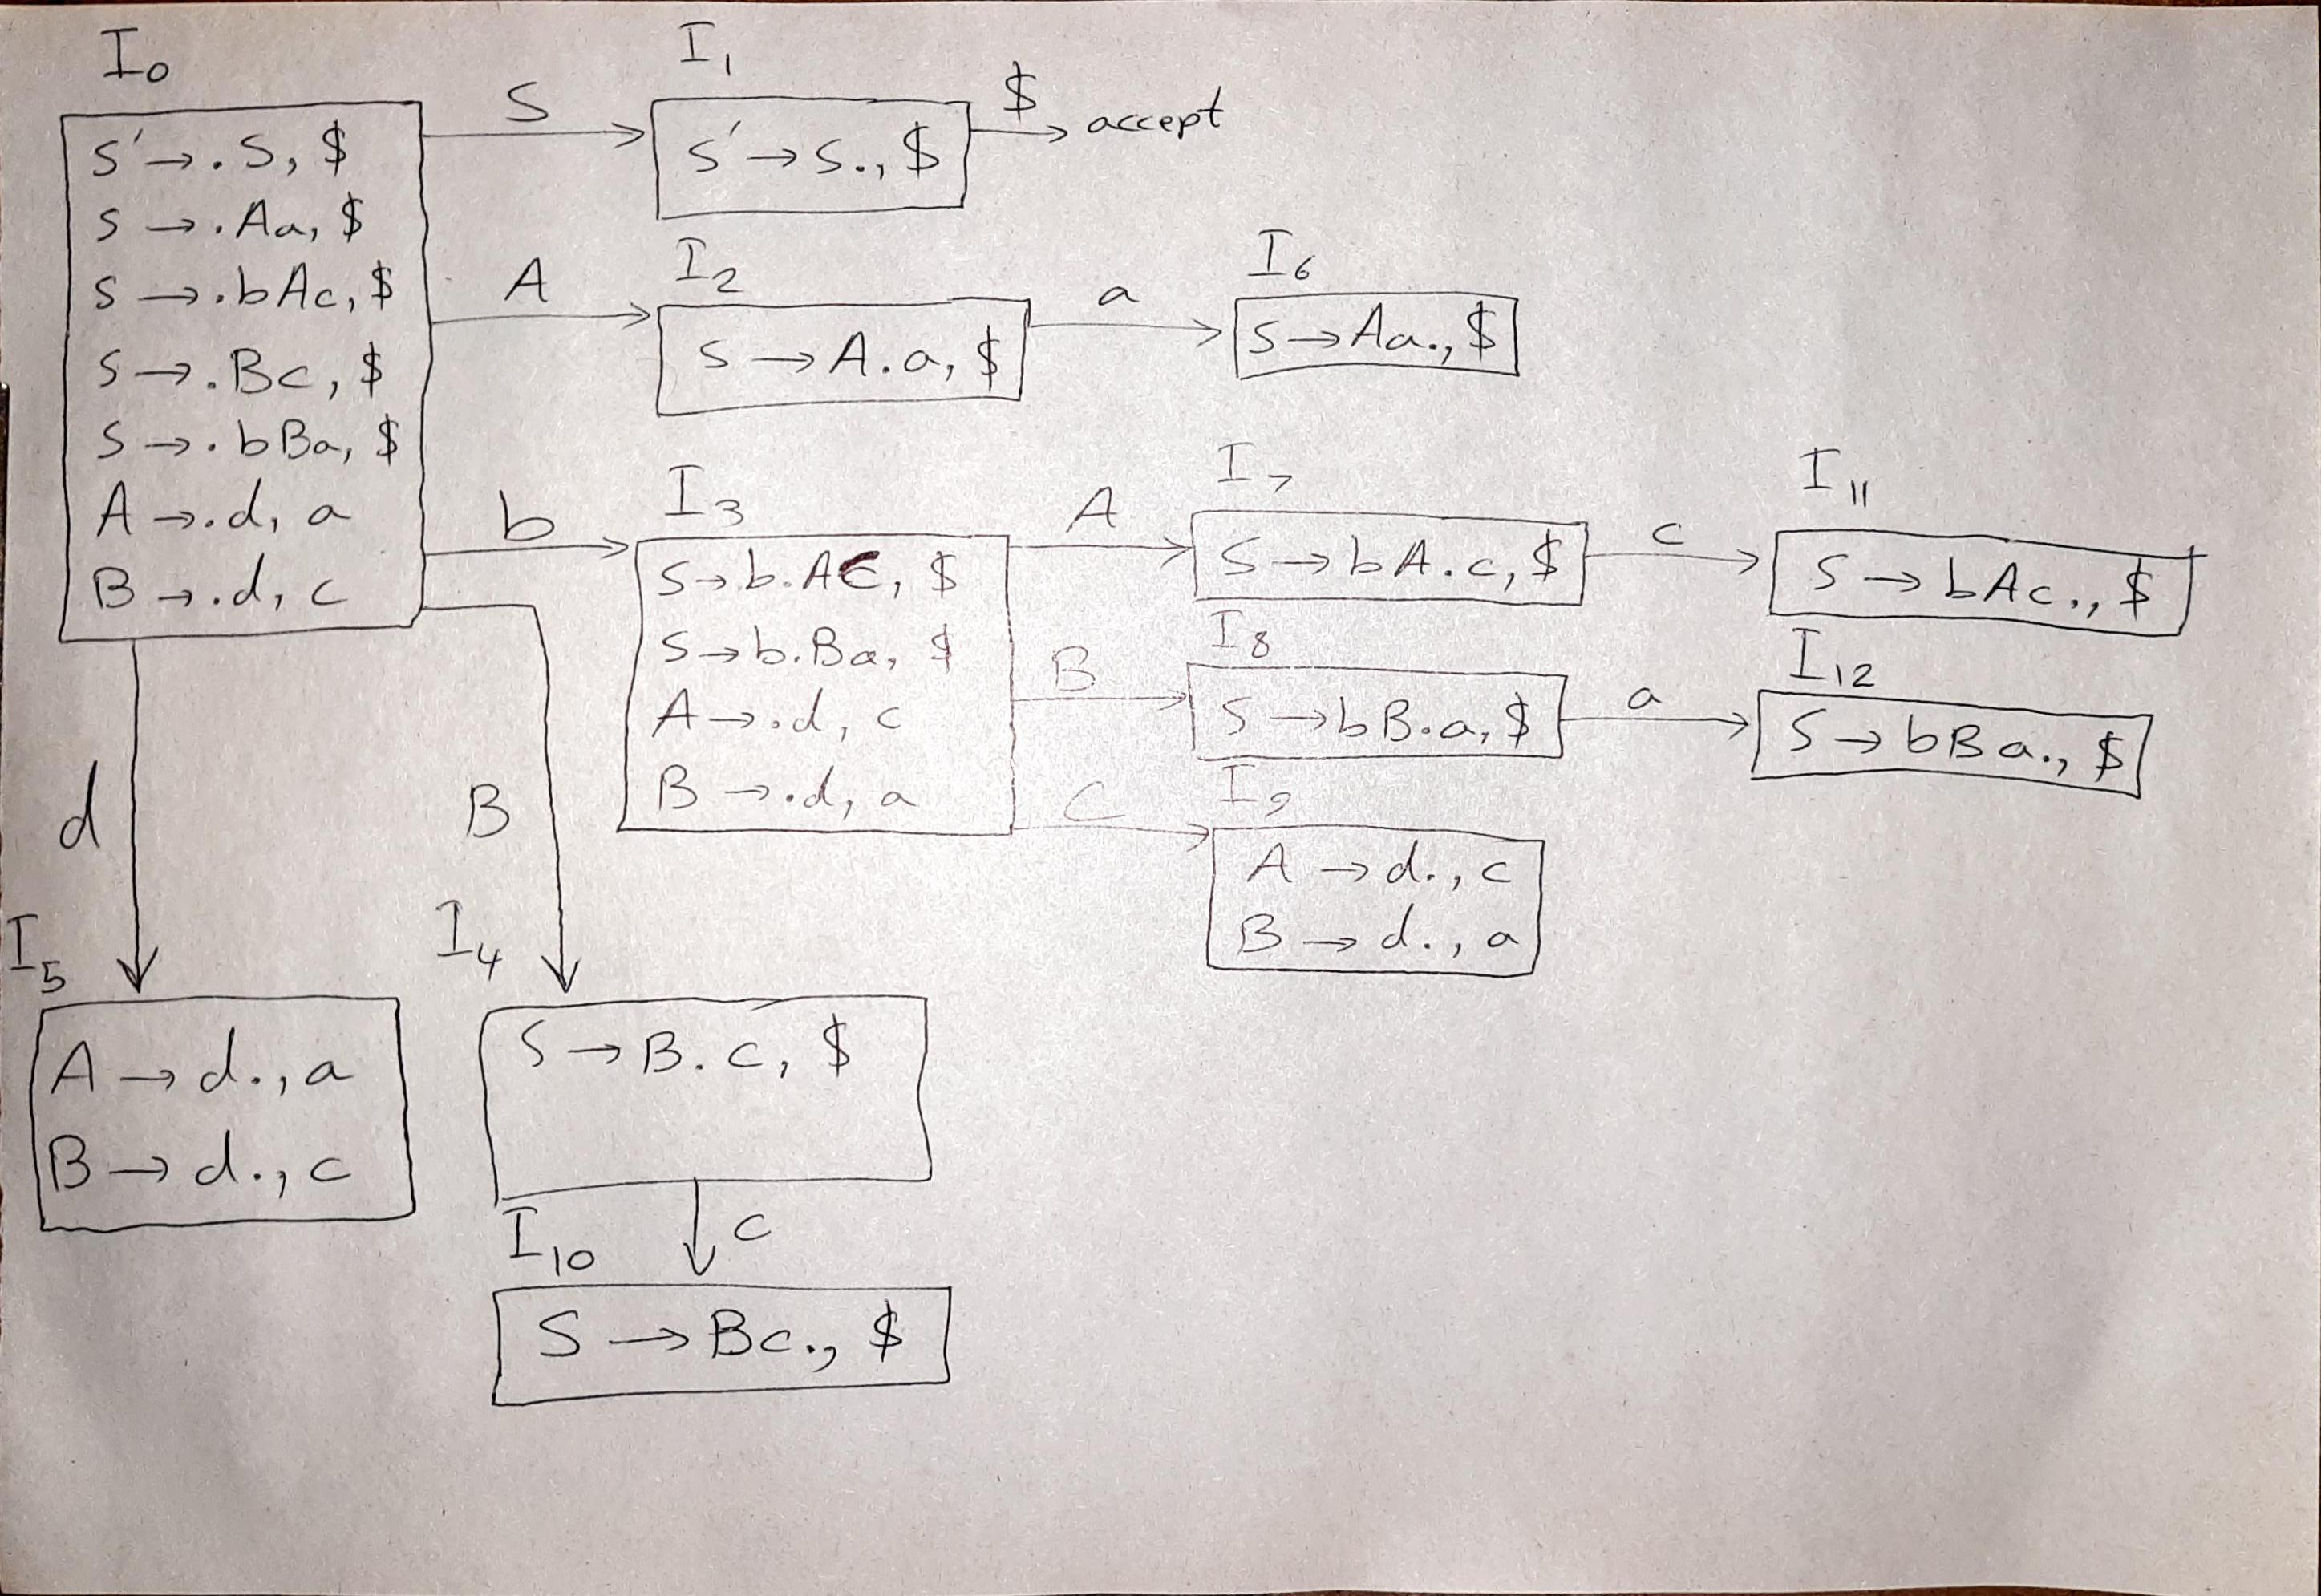
\includegraphics[width=1.0\textwidth]{figures/9b.jpg}
    \caption
	{}
    \label{fig:fig1}
\end{figure}

همانطور که در ماشین حالت بالا مشخص است، هیچ استیتی دارای کانفلیکت نیست. اما برای تجزیه‌ی $LALR(1)$ باید استیت‌های 5 و 6 ادغام شوند که باعث ایجاد کانفلیکت \lr{reduce-reduce} می‌شود.


\section{}%10
\subsection{آ}
ابتدا سمبل‌های مختلف گرامر را به شکل زیر دسته‌بندی می‌کنیم.
\begin{latin}
\begin{table}[H]
\begin{tabular}{|l|c|}
\hline
Terminal     & $\left\{ (, \mathbb{,}, ), a, b, \$ \right\} $ \\ \hline
Non-terminal & $\left\{ S ^ \prime, S, A \right\}$            \\ \hline
\end{tabular}
\end{table}
\end{latin}
که $S^\prime$ استیت شروع است.\\

با توجه به اینکه $GOTO(0, S)$ برابر 1 است پس داریم:
\begin{latin}
$\\
S^\prime \longrightarrow S
$
\end{latin}

با توجه به اینکه $GOTO(0, A)$ برابر 3 است، می‌دانیم که یکی از \lr{production} با \lr{A} آغاز می‌شود و از آن‌جایی که تنها \lr{r2} در استیت 3 دارای طول 1 است داریم:
\begin{latin}
$\\
S \longrightarrow A
$
\end{latin}

با توجه به استیت‌های 0، 6، 8، 9، 10 و مقادیر $GOTO$، $ACTION$، $shift$ و $reduce$شان داریم:
\begin{latin}
$\\
S \longrightarrow (A, S)
$
\end{latin}
با توجه به استیت‌های 0، 4، و 7 داریم:
\begin{latin}
$\\
A \longrightarrow a S
$
\end{latin}

و با توجه به استیت‌های 0، و 5 داریم:
\begin{latin}
$\\
A \longrightarrow b
$
\end{latin}

پس در نهایت گرامری كه جداول سوال از روی آن توليد شده است، به صورت زیر است:
\begin{latin}
$\\
S ^ \prime \longrightarrow S \\
S \longrightarrow (A, S) \\
S \longrightarrow A \\
A \longrightarrow a S \\
A \longrightarrow b
$
\end{latin}

\subsection{ب}
مراحل تجزیه به صورت زیر می‌باشد:
\begin{latin}
% Please add the following required packages to your document preamble:
% \usepackage[table,xcdraw]{xcolor}
% If you use beamer only pass "xcolor=table" option, i.e. \documentclass[xcolor=table]{beamer}
\begin{table}[H]
\begin{tabular}{|llll|}
\hline
\multicolumn{4}{|c|}{\textbf{Trace}}                                                                                                                                                    \\ \hline
\multicolumn{1}{|c|}{\textbf{Step}} & \multicolumn{1}{c|}{\textbf{Stack}}                                & \multicolumn{1}{c|}{\textbf{Input}}   & \multicolumn{1}{c|}{\textbf{Action}} \\ \hline
\multicolumn{1}{|l|}{1}             & \multicolumn{1}{l|}{{\color[HTML]{0000FF} 0}}                      & \multicolumn{1}{l|}{( a a b , b ) \$} & s2                                   \\ \hline
\multicolumn{1}{|l|}{2}             & \multicolumn{1}{l|}{{\color[HTML]{0000FF} 0 ( 2}}                  & \multicolumn{1}{l|}{a a b , b ) \$}   & s4                                   \\ \hline
\multicolumn{1}{|l|}{3}             & \multicolumn{1}{l|}{{\color[HTML]{0000FF} 0 ( 2 a 4}}              & \multicolumn{1}{l|}{a b , b ) \$}     & s4                                   \\ \hline
\multicolumn{1}{|l|}{4}             & \multicolumn{1}{l|}{{\color[HTML]{0000FF} 0 ( 2 a 4 a 4}}          & \multicolumn{1}{l|}{b , b ) \$}       & s5                                   \\ \hline
\multicolumn{1}{|l|}{5}             & \multicolumn{1}{l|}{{\color[HTML]{0000FF} 0 ( 2 a 4 a 4 b 5}}      & \multicolumn{1}{l|}{, b ) \$}         & r4                                   \\ \hline
\multicolumn{1}{|l|}{6}             & \multicolumn{1}{l|}{{\color[HTML]{0000FF} 0 ( 2 a 4 a 4 A}}        & \multicolumn{1}{l|}{, b ) \$}         & {\color[HTML]{0000FF} 3}             \\ \hline
\multicolumn{1}{|l|}{7}             & \multicolumn{1}{l|}{{\color[HTML]{0000FF} 0 ( 2 a 4 a 4 A 3}}      & \multicolumn{1}{l|}{, b ) \$}         & r2                                   \\ \hline
\multicolumn{1}{|l|}{8}             & \multicolumn{1}{l|}{{\color[HTML]{0000FF} 0 ( 2 a 4 a 4 S}}        & \multicolumn{1}{l|}{, b ) \$}         & {\color[HTML]{0000FF} 7}             \\ \hline
\multicolumn{1}{|l|}{9}             & \multicolumn{1}{l|}{{\color[HTML]{0000FF} 0 ( 2 a 4 a 4 S 7}}      & \multicolumn{1}{l|}{, b ) \$}         & r3                                   \\ \hline
\multicolumn{1}{|l|}{10}            & \multicolumn{1}{l|}{{\color[HTML]{0000FF} 0 ( 2 a 4 A}}            & \multicolumn{1}{l|}{, b ) \$}         & {\color[HTML]{0000FF} 3}             \\ \hline
\multicolumn{1}{|l|}{11}            & \multicolumn{1}{l|}{{\color[HTML]{0000FF} 0 ( 2 a 4 A 3}}          & \multicolumn{1}{l|}{, b ) \$}         & r2                                   \\ \hline
\multicolumn{1}{|l|}{12}            & \multicolumn{1}{l|}{{\color[HTML]{0000FF} 0 ( 2 a 4 S}}            & \multicolumn{1}{l|}{, b ) \$}         & {\color[HTML]{0000FF} 7}             \\ \hline
\multicolumn{1}{|l|}{13}            & \multicolumn{1}{l|}{{\color[HTML]{0000FF} 0 ( 2 a 4 S 7}}          & \multicolumn{1}{l|}{, b ) \$}         & r3                                   \\ \hline
\multicolumn{1}{|l|}{14}            & \multicolumn{1}{l|}{{\color[HTML]{0000FF} 0 ( 2 A}}                & \multicolumn{1}{l|}{, b ) \$}         & {\color[HTML]{0000FF} 6}             \\ \hline
\multicolumn{1}{|l|}{15}            & \multicolumn{1}{l|}{{\color[HTML]{0000FF} 0 ( 2 A 6}}              & \multicolumn{1}{l|}{, b ) \$}         & s8                                   \\ \hline
\multicolumn{1}{|l|}{16}            & \multicolumn{1}{l|}{{\color[HTML]{0000FF} 0 ( 2 A 6 , 8}}          & \multicolumn{1}{l|}{b ) \$}           & s5                                   \\ \hline
\multicolumn{1}{|l|}{17}            & \multicolumn{1}{l|}{{\color[HTML]{0000FF} 0 ( 2 A 6 , 8 b 5}}      & \multicolumn{1}{l|}{) \$}             & r4                                   \\ \hline
\multicolumn{1}{|l|}{18}            & \multicolumn{1}{l|}{{\color[HTML]{0000FF} 0 ( 2 A 6 , 8 A}}        & \multicolumn{1}{l|}{) \$}             & {\color[HTML]{0000FF} 3}             \\ \hline
\multicolumn{1}{|l|}{19}            & \multicolumn{1}{l|}{{\color[HTML]{0000FF} 0 ( 2 A 6 , 8 A 3}}      & \multicolumn{1}{l|}{) \$}             & r2                                   \\ \hline
\multicolumn{1}{|l|}{20}            & \multicolumn{1}{l|}{{\color[HTML]{0000FF} 0 ( 2 A 6 , 8 S}}        & \multicolumn{1}{l|}{) \$}             & {\color[HTML]{0000FF} 9}             \\ \hline
\multicolumn{1}{|l|}{21}            & \multicolumn{1}{l|}{{\color[HTML]{0000FF} 0 ( 2 A 6 , 8 S 9}}      & \multicolumn{1}{l|}{) \$}             & s10                                  \\ \hline
\multicolumn{1}{|l|}{22}            & \multicolumn{1}{l|}{{\color[HTML]{0000FF} 0 ( 2 A 6 , 8 S 9 ) 10}} & \multicolumn{1}{l|}{\$}               & r1                                   \\ \hline
\multicolumn{1}{|l|}{23}            & \multicolumn{1}{l|}{{\color[HTML]{0000FF} 0 S}}                    & \multicolumn{1}{l|}{\$}               & {\color[HTML]{0000FF} 1}             \\ \hline
\multicolumn{1}{|l|}{24}            & \multicolumn{1}{l|}{{\color[HTML]{0000FF} 0 S 1}}                  & \multicolumn{1}{l|}{\$}               & {\color[HTML]{008000} acc}           \\ \hline
\end{tabular}
\end{table}
\end{latin}



%%%%%%%%%%%%%%%%%%%%%%%%%%%%%%%%%
%------------------------------------------------------------------------------------------
\end{document}